%\documentclass[12pt,a4paper,onecolumn,twoside]{elsarticle}
\documentclass[12pt,a4paper,onecolumn,twoside]{article}

\usepackage{vmargin, xspace}
\usepackage[numbers]{natbib}

\usepackage{url}
\usepackage[english]{babel}

\usepackage[absolute]{textpos}
\usepackage{setspace}

\usepackage{graphicx}
\DeclareGraphicsExtensions{.eps,.png,.pdf}

\usepackage{amsmath,amssymb}
\usepackage{graphicx,subfigure}
\usepackage{hhline}
\usepackage{arydshln}
\usepackage{myacronym}
\usepackage{multirow}

% My adapted version of pythonlisting
\usepackage{color}
\usepackage[procnames]{listings}
\usepackage{textcomp}
\usepackage{setspace}
\usepackage{palatino}
\renewcommand{\lstlistlistingname}{Code Listings}
\renewcommand{\lstlistingname}{Code Listing}
\definecolor{gray}{gray}{0.5}
\definecolor{green}{rgb}{0,0.5,0}
\definecolor{lightgreen}{rgb}{0,0.7,0}
\definecolor{purple}{rgb}{0.5,0,0.5}
\definecolor{darkred}{rgb}{0.5,0,0}
\definecolor{orange}{rgb}{1,0.5,0}
%\lstnewenvironment{python}[1][]{
%\lstset{
%numbers=left,
%numberstyle=\sffamily\scriptsize,
%numberblanklines=false,
%showstringspaces=false,
%language=python,
%basicstyle=\ttfamily\small\setstretch{1},
%stringstyle=\color{green},
%showstringspaces=false,
%alsoletter={1234567890},
%otherkeywords={\ , \}, \{},
%keywordstyle=\color{blue},
%emph={access,and,as,break,class,continue,def,del,elif,else,%
%except,exec,finally,for,from,global,if,import,in,is,%
%lambda,not,or,pass,print,raise,return,try,while,assert},
%emphstyle=\color{orange}\bfseries,
%emph={[2]self},
%emphstyle=[2]\color{gray},
%emph={[4]ArithmeticError,AssertionError,AttributeError,BaseException,%
%DeprecationWarning,EOFError,Ellipsis,EnvironmentError,Exception,%
%False,FloatingPointError,FutureWarning,GeneratorExit,IOError,%
%ImportError,ImportWarning,IndentationError,IndexError,KeyError,%
%KeyboardInterrupt,LookupError,MemoryError,NameError,None,%
%NotImplemented,NotImplementedError,OSError,OverflowError,%
%PendingDeprecationWarning,ReferenceError,RuntimeError,RuntimeWarning,%
%StandardError,StopIteration,SyntaxError,SyntaxWarning,SystemError,%
%SystemExit,TabError,True,TypeError,UnboundLocalError,UnicodeDecodeError,%
%UnicodeEncodeError,UnicodeError,UnicodeTranslateError,UnicodeWarning,%
%UserWarning,ValueError,Warning,ZeroDivisionError,abs,all,any,apply,%
%basestring,bool,buffer,callable,chr,classmethod,cmp,coerce,compile,%
%complex,copyright,credits,delattr,dict,dir,divmod,enumerate,eval,%
%execfile,exit,file,filter,float,frozenset,getattr,globals,hasattr,%
%hash,help,hex,id,input,int,intern,isinstance,issubclass,iter,len,%
%license,list,locals,long,map,max,min,object,oct,open,ord,pow,property,%
%quit,range,raw_input,reduce,reload,repr,reversed,round,set,setattr,%
%slice,sorted,staticmethod,str,sum,super,tuple,type,unichr,unicode,%
%vars,xrange,zip},
%emphstyle=[4]\color{purple}\bfseries,
%upquote=true,
%morecomment=[s][\color{lightgreen}]{"""}{"""},
%commentstyle=\color{red}\slshape,
%literate={>>>}{\textbf{\textcolor{darkred}{>{>}>}}}3%
%         {...}{{\textcolor{gray}{...}}}3,
%procnamekeys={def,class},
%procnamestyle=\color{blue}\textbf,
%framexleftmargin=1mm, framextopmargin=1mm, frame=shadowbox,
%rulesepcolor=\color{blue},#1
%}}{}

% Initialise the listing settings
\lstset{
numbers=left,
numberstyle=\sffamily\scriptsize,
numberblanklines=false,
showstringspaces=false,
language=python,
basicstyle=\ttfamily\footnotesize\setstretch{1},
stringstyle=\color{green},
showstringspaces=false,
alsoletter={1234567890},
otherkeywords={\ , \}, \{},
keywordstyle=\color{blue},
emph={access,and,as,break,class,continue,def,del,elif,else,%
except,exec,finally,for,from,global,if,import,in,is,%
lambda,not,or,pass,print,raise,return,try,while,assert},
emphstyle=\color{orange}\bfseries,
emph={[2]self},
emphstyle=[2]\color{gray},
emph={[4]ArithmeticError,AssertionError,AttributeError,BaseException,%
DeprecationWarning,EOFError,Ellipsis,EnvironmentError,Exception,%
False,FloatingPointError,FutureWarning,GeneratorExit,IOError,%
ImportError,ImportWarning,IndentationError,IndexError,KeyError,%
KeyboardInterrupt,LookupError,MemoryError,NameError,None,%
NotImplemented,NotImplementedError,OSError,OverflowError,%
PendingDeprecationWarning,ReferenceError,RuntimeError,RuntimeWarning,%
StandardError,StopIteration,SyntaxError,SyntaxWarning,SystemError,%
SystemExit,TabError,True,TypeError,UnboundLocalError,UnicodeDecodeError,%
UnicodeEncodeError,UnicodeError,UnicodeTranslateError,UnicodeWarning,%
UserWarning,ValueError,Warning,ZeroDivisionError,abs,all,any,apply,%
basestring,bool,buffer,callable,chr,classmethod,cmp,coerce,compile,%
complex,copyright,credits,delattr,dict,dir,divmod,enumerate,eval,%
execfile,exit,file,filter,float,frozenset,getattr,globals,hasattr,%
hash,help,hex,id,input,int,intern,isinstance,issubclass,iter,len,%
license,list,locals,long,map,max,min,object,oct,open,ord,pow,property,%
quit,range,raw_input,reduce,reload,repr,reversed,round,set,setattr,%
slice,sorted,staticmethod,str,sum,super,tuple,type,unichr,unicode,%
vars,xrange,zip},
emphstyle=[4]\color{purple}\bfseries,
upquote=true,
morecomment=[s][\color{lightgreen}]{"""}{"""},
commentstyle=\color{red}\slshape,
literate={>>>}{\textbf{\textcolor{darkred}{>{>}>}}}3%
         {...}{{\textcolor{gray}{...}}}3,
procnamekeys={def,class},
procnamestyle=\color{blue}\textbf,
framexleftmargin=1mm, framextopmargin=1mm, frame=shadowbox,
rulesepcolor=\color{blue}
}
\usepackage{comment}

\newcommand{\eqnref}[1]{\eqref{#1}}

\newcommand{\scnref}[1]{section \ref{#1}}
\newcommand{\Scnref}[1]{Section \ref{#1}}

\newcommand{\sbsref}[1]{\S \ref{#1}}
\newcommand{\Sbsref}[1]{Section \ref{#1}}

\newcommand{\figref}[1]{figure \ref{#1}}
\newcommand{\Figref}[1]{Figure \ref{#1}}

\newcommand{\tabref}[1]{Table \ref{#1}}
\newcommand{\Tabref}[1]{Table \ref{#1}}

\newcommand{\twosubs}[2]{\begin{matrix} \\[-14pt] \scriptstyle #1 \\[-3pt] \scriptstyle #2 \end{matrix}} 

% Examples path (added by IRD 14/4/2011)
\newcommand{\dippypath}[0]{C:/COIN}

\begin{document}

\begin{titlepage}
\ 
\setlength{\TPHorizModule}{1cm}
\setlength{\TPVertModule}{1cm}
\begin{textblock}{8.79}(8.655,11.5)
\begin{center}
\textbf{
\begin{Large}
\begin{onehalfspace}
Dippy -- a simplified interface\\[-6pt] for advanced mixed-integer \\[-6pt] programming\\[3pt]
\end{onehalfspace}
\end{Large}
By Dr Michael O'Sullivan, Dr Cameron Walker, Qi-Shan Lim,%
Iain Dunning, Dr Stuart Mitchell and Assoc Prof Ted Ralphs\\[3pt]
February 2011\\
Report, University of Auckland Faculty of Engineering, no. ???\\
%ISSN 1179-528X % Print version
ISSN 1178-3680 % Electronic version
}
\end{center}
\end{textblock}
\vfill
\end{titlepage}

\title{
Dippy -- a simplified interface for advanced mixed-integer programming
}

\author{Michael O'Sullivan\footnotemark, \ 
				Qi-Shan Lim, \
        Cameron Walker, \
        Iain Dunning\\
        {\it \small Department of Engineering Science, The University of Auckland, Auckland, New Zealand}\\
        Stuart Mitchell\\
        {\it \small Stuart Mitchell Consulting, Auckland, New Zealand}\\
        Ted Ralphs\\
        {\it \small Department of Industrial Engineering, Lehigh University, Pennsylvania, USA}}

\date{\today}

\maketitle

\def\thefootnote{\fnsymbol{footnote}}
\footnotetext[1]{\begin{tabular}[t]{@{}l}
                 \,Corresponding author.\\
                 {\it E-mail address:} michael.osullivan@auckland.ac.nz (M. J. O'Sullivan)
                 \end{tabular}}
\def\thefootnote{\arabic{footnote}}
          
\pagestyle{plain} \thispagestyle{empty}
\pagenumbering{arabic}

\acrodef{MILP}{mixed-integer linear programming}
\acrodef{DIP}{Decomposition for Integer Programming}
\acrodef{CGL}{Cut Generator Library}
\acrodef{OSI}{Open Solver Interface}
\acrodef{DP}{dynamic programming}
\acrodef{TSP}{travelling salesperson}

\subsection*{Abstract}
Mathematical modelling languages such as AMPL, GAMS, and Xpress-MP enable mathematical models such as mixed-integer linear programmes (MILPs) to be expressed clearly for solution in solvers such as CPLEX, MINOS and Gurobi.
However, some models are sufficiently difficult that they cannot be solved using ``out-of-the-box'' solvers, and customisation of the solver framework to exploit model-specific structure is required.
Many solvers, including CPLEX, Symphony and DIP, enable this customisation by providing ``callback functions'' that are called at key steps in the solution of a model.
This approach traditionally involves either expressing the mathematical formulation in a low-level language, such as C++ or Java, or implementing a complicated indexing scheme to be able to track model components, such as variables and constraints, between the mathematical modelling language and the solver's callback framework.

In this paper we present Dippy, a combination of the Python-based mathematical modelling language PuLP and the open source solver DIP. 
Dippy provides the power of callback functions, but without sacrificing the usability and flexibility of modelling languages.
We discuss the link between PuLP and DIP and give examples of how advanced solving techniques can be expressed concisely and intuitively in Dippy.

\section{Introduction} \label{scn:intro}
%Using a high-level modelling language such as AMPL, GAMS, Xpress-Mp or OPL Studio enables Operations Research practitioners to express complicated \ac{MILP} problems relatively quickly and naturally compared to expressing them with a traditional computer programming language.
Using a high-level modelling language such as AMPL, GAMS, Xpress-MP or OPL Studio enables Operations Research practitioners to express complicated \ac{MILP} problems quickly and naturally.
Once defined in one of these high-level languages, the \ac{MILP} can be solved using one of a number of solvers.
However these solvers are not effective for all problem instances due to the computational difficulties associated with solving \ac{MILP}s (an NP-Hard class of problems).
Despite steadily increasing computing power and algorithmic improvements for the solution of \ac{MILP}s in general, in many cases problem-specific techniques need to be included in the solution process to solve problems of a useful size in any reasonable time.

Both commercial solvers -- such as CPLEX and Gurobi -- and open source solvers -- such as CBC, Symphony and \acs{DIP} (all from the COIN-OR repository \cite{coin_or}) -- provide callback functions that allow user-defined routines to be included in the solution framework.
To make use of these callback functions the user must first create their \ac{MILP} problem in a low-level computer programming language (C, C++ or Java for CPLEX, C, C++, C\#, Java or Python for Gurobi, C or C++ for CBC, Symphony or \acs{DIP}).
%While defining their problem they need to create structures to keep track of appropriate constraints and/or variables for later use in their user-defined routines.
As part of the problem definition, it is necessary to create structures to keep track of the constraints and\slash{}or variables.
Problem definition in C\slash{}C++\slash{}Java for a \ac{MILP} problem of any reasonable size and complexity is a major undertaking and thus a major barrier to the development of customised \ac{MILP} frameworks by both practitioners and researchers.

Given the difficulty in defining a \ac{MILP} problem in a low-level language, another alternative for problem formulation is to use a high-level mathematical modelling language.
By carefully constructing an indexing scheme, constraints and\slash{}or variables in the high-level language can be identified in the low-level callback functions.
However implementing the indexing scheme can be as difficult as using the low-level language to define the problem in the first place and does little to remove the barrier to solution development.

The purpose of the research presented here is to demonstrate a tool, Dippy, that supports easy experimentation with and customisation of advanced \ac{MILP} solution frameworks. 
To achieve this aim we needed to:
\begin{enumerate}
\item provide a modern high-level modelling system that enables users to quickly and easily describe their \ac{MILP} problems;
\item enable simple identification of constraints and variables in user-defined routines in the solution framework.
\end{enumerate}
The first requirement is satisfied by the modelling language PuLP~\cite{pulp}.
Dippy extends PuLP to use the \ac{DIP} solver, and enables user-defined routines, implemented using Python and PuLP, to be accessed by the \ac{DIP} callback functions. This approach enables constraints or variables defined in the \ac{MILP} model to be easily accessed using PuLP in the user-defined routines.
In addition to this, \ac{DIP} is implemented so that the \ac{MILP} problem is defined the same way whether branch-and-cut or branch-price-and-cut is being used -- it hides the implementation of the master problem and subproblems.
This makes it very easy to switch between the two approaches when experimenting with solution methods.
All this functionality combines to overcome the barrier described previously and provides researchers, practitioners and students with a simple and integrated way of describing problems and customising the solution framework.

The rest of this article is structured as follows.
In \scnref{scn:overview} we provide an overview of the interface between PuLP and \ac{DIP}, including a description of the callback functions available in Python from \ac{DIP}.
In \scnref{scn:techs} we describe how Dippy enables experimentation with improvements to \ac{DIP}'s \ac{MILP} solution framework by showing example code for a common problem.
We conclude in \scnref{scn:concl} where we discuss how this project enhances the ability of researchers to experiment with approaches for solving difficult \ac{MILP} problems. We also demonstrate that \ac{DIP} (via PuLP and Dippy) is competitive with leading commercial (Gurobi) and open source (CBC) solvers.


\section{Combining \ac{DIP} and PuLP} \label{scn:overview}
Dippy is the primarily the ``glue'' between two different technologies: PuLP and DIP.

PuLP~\cite{pulp} is a mathematical modelling language and toolkit that uses Python.
Users can define \ac{MILP} problems and solve them using a variety of solvers including CPLEX, Gurobi and CBC.
PuLP's solver interface is modular and thus can be easily extended to use other solvers such as \ac{DIP}.
For more details on PuLP see the PuLP project in the COIN-OR repository~\cite{coin_or}.

\acf{DIP}~\cite{decomp04} provides a framework for solving \ac{MILP} problems using 3 different methods\footnote{The skeleton for a fourth method (branch, relax and cut) exists in \ac{DIP}, but this method is not yet implemented.}:
\begin{enumerate}
	\item ``branch-and-cut'',
	\item ``branch-price-and-cut'',
	\item ``decompose-and-cut''.
\end{enumerate}
In this paper we will restrict our attention to branch-and-cut and branch-price-and-cut.

Branch-and-cut uses the classic branch-and-bound approach for solving \ac{MILP}s combined with the cutting plane method for removing fractionality encountered at the branch-and-bound nodes.
This framework is the basis of many state-of-the-art \ac{MILP} solvers including Gurobi and CBC.
\ac{DIP} provides callback functions that allow users to customise the solution process by adding their own cuts and running heuristics at each node.

Branch-price-and-cut uses Dantzig-Wolfe decomposition to split a large \ac{MILP} problem into a master problem and one or more subproblems.
The subproblems solve a pricing problem, defined using the master problem dual values, to add new variables to the master problem.
Branch-and-cut is then used on the master problem.

The cut generation and heuristic callback functions mentioned previously can also be used for branch-price-and-cut.
Extra callback functions enable the user to define their own routines for finding initial variables to include in the master problem and for solving the subproblems to generate new master problem variables.
For details on the methods and callback functions provided by \ac{DIP} see~\cite{decomp04}.

In addition to the \ac{DIP} callback functions (see \sbsref{sbs:callbacks}), we modified DIP to add another callback function that enables user-defined branching in \ac{DIP} and so can be used in any of the solution methods within \ac{DIP}.

\subsection{Callback Functions} \label{sbs:callbacks}

\begin{sloppypar}\paragraph{Advanced Branching}
We replaced \lstinline{chooseBranchVar} in the \ac{DIP} source with a new function \lstinline{chooseBranchSet}. 
This is a significant change to branching in DIP that makes it possible for the user to define:
\begin{itemize}
\item a {\it down} set of variables with (lower and upper) bounds that will be enforced in the down node of the branch; and,
\item an {\it up} set of variables with bounds that will be enforced in the up node of the branch.
\end{itemize}
A typical variable branch on an integer variable $x$ with integer bounds $l$ and $u$ and fractional value $\alpha$ can be implemented by:
\begin{enumerate}
\item choosing the down set to be $\{ x \}$ with bounds $l$ and $\lfloor \alpha \rfloor$;
\item choosing the up set to be $\{ x \}$ with bounds of $\lceil \alpha \rceil$ and $u$.
\end{enumerate}
However, other branching methods may use advanced branching techniques such as the one demonstrated in \sbsref{sbs:branch}.
From \ac{DIP}, \lstinline{chooseBranchSet} calls \lstinline{branch_method} in Dippy.\end{sloppypar}

\begin{sloppypar}\paragraph{Customised Cuts} % sloppypar deals with the line break issue by doing what you'd expect - pushing it to next line, bigger gaps
We modified \lstinline{generateCuts} (in the \ac{DIP} source) to call \lstinline{generate_cuts} in Dippy.
This enables the user to examine a solution and generate any customised cuts as necessary.
We also modified \lstinline{APPisUserFeasible} to call \lstinline{is_solution_feasible} in Dippy, enabling users to check solutions for feasibility with respect to customised cuts.\end{sloppypar}

\begin{sloppypar}\paragraph{Customised Columns (Solutions to Subproblems)}
We modified the \ac{DIP} function \lstinline{solveRelaxed} to call \lstinline{relaxed_solver} in Dippy.
This enables the user to utilise the master problem dual variables to produce solutions to subproblems (and so add columns to the master problem) using customised methods.
We also modified \lstinline{generateInitVars} to call \lstinline{init_vars} in Dippy, enabling users to customise the generation of initial columns for the master problem.\end{sloppypar}

\begin{sloppypar}\paragraph{Heuristics}
We modified \lstinline{APPheuristics} (\ac{DIP}) to call \lstinline{heuristics} (Dippy).
This enables the user to define customised heuristics at each node in the branch-and-bound tree (including the root node).\end{sloppypar}

\subsection{Interface}

The interface between Dippy (in Python) and DIP (in C++) is summarised in \figref{fig:interface}.
\begin{figure}[htp]
%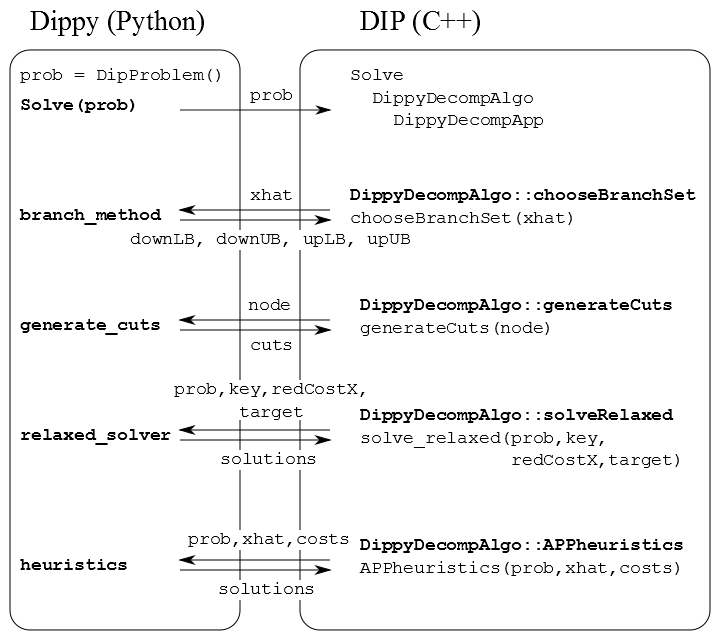
\includegraphics[bb=0 0 960 720,scale=0.45]{img/interface.png}
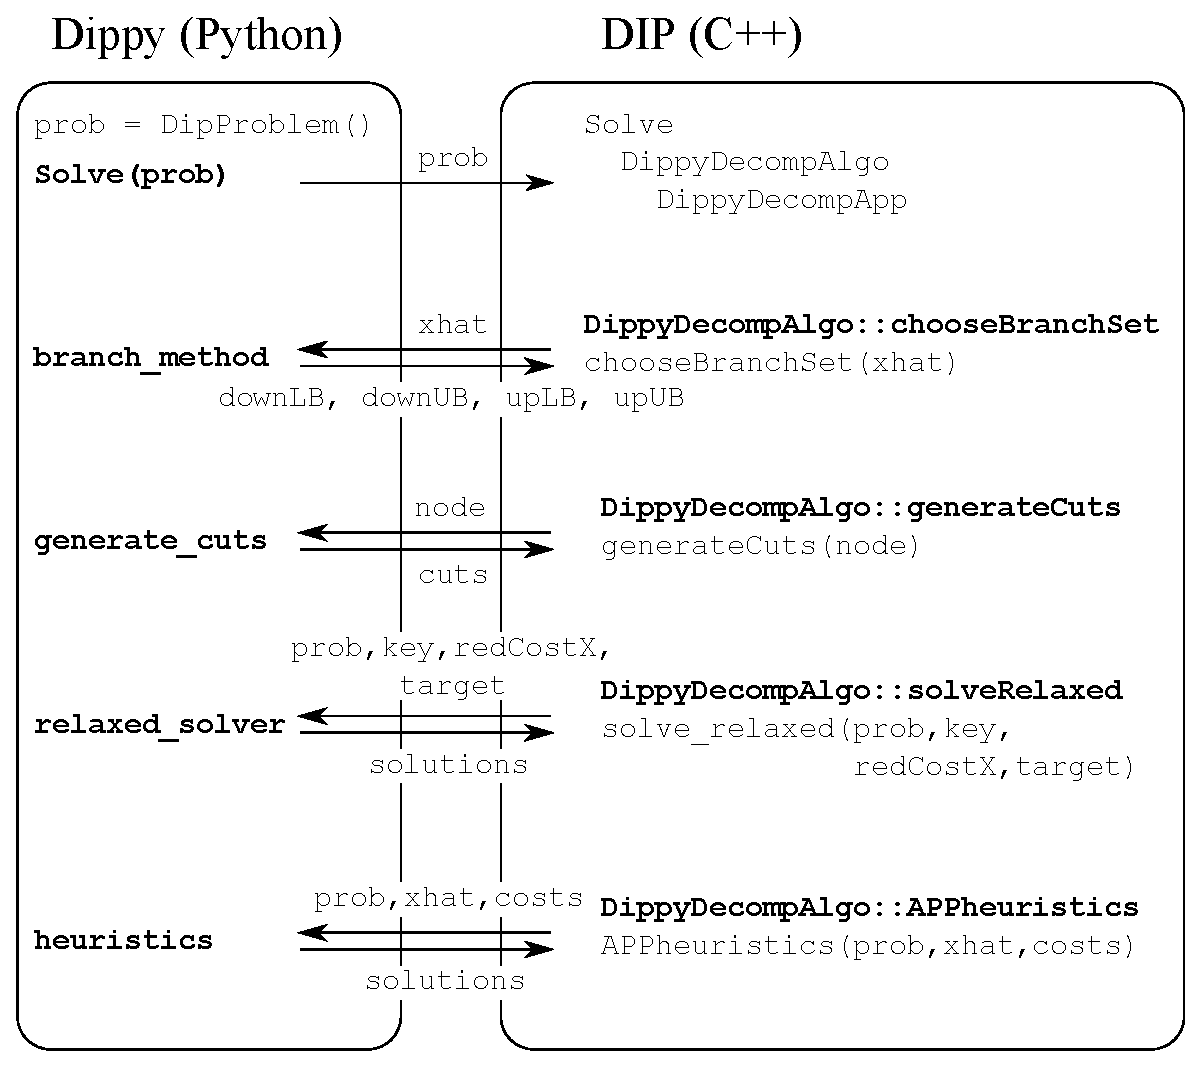
\includegraphics[scale=0.70]{img/diagram.eps}
\caption{Key components of interface between Dippy and DIP.} \label{fig:interface}
\end{figure}

\begin{sloppypar}The \ac{MILP} is defined as a \lstinline{DipProblem} and then solved using the \lstinline{Solve} command in Dippy, that passes the Python \lstinline{DipProblem} object, \lstinline{prob}, to DIP in C++.
\ac{DIP} \lstinline{Solve} creates a \lstinline{DippyDecompAlgo} object that contains a \lstinline{DippyDecompApp} object, both of which are populated by data from \lstinline{prob}.
As \ac{DIP} \lstinline{Solve} proceeds branches are created by the \lstinline{DippyDecompAlgo} object using \lstinline{chooseBranchSet} which passes the current node's fractional solution \lstinline{xhat} back to the \lstinline{branch_method} function in the \lstinline{DipProblem} object \lstinline{prob}.
This function generates lower and upper bounds for the ``down'' and ``up'' branches and returns to \lstinline{DippyDecompAlgo::chooseBranchSet}.
When \ac{DIP} generates cuts, it uses the \lstinline{DippyDecompApp} object's \lstinline{generateCuts} function which passes the current node \lstinline{node} to the \lstinline{DipProblem} object's \lstinline{generate_cuts} function.
This function generates any customised cuts and returns a list, \lstinline{cuts}, back to \lstinline{DippyDecompApp::generateCuts}.
These interfaces are replicated for the other callback functions provided by Dippy.\end{sloppypar}


\section{Dippy in Practice} \label{scn:techs}
We will use the Bin Packing Problem to demonstrate the implementation of customised branching rules, custom cuts, heuristics, and a column generation algorithm.

The solution of the problem determines which, of $m$ bins, to use and also places $n$ items of various sizes into the bins in a way that (in this version) minimises the wasted capacity of the bins.
Each item $j=1, \ldots, n$ has a size $s_j$ and each bin has capacity $C$.
Extensions of this problem arise often in \ac{MILP} in problems including network design and rostering.

The \ac{MILP} formulation of the bin packing problem is straightforward.
The decision variables are
\begin{align*}
x_{ij} &= \begin{cases} 1 & \text{if item $j$ is placed in bin $i$} \\
0 & \text{otherwise} \end{cases} \\
y_i &= \begin{cases} 1 & \text{if bin $i$ is used} \\
0 & \text{otherwise} \end{cases} \\
w_i &= \text{ ``wasted'' capacity in bin $i$}
\end{align*}
and the formulation is
\[
\begin{array}{rr@{\ }ll}
       \min & \displaystyle \sum_{i=1}^m w_i \\
\text{s.t.} & \displaystyle \sum_{i=1}^m x_{ij}           & = 1, j = 1, \ldots, n      & \text{ (each item packed)} \\
            & \displaystyle \sum_{j=1}^n s_j x_{ij} + w_i & = C y_i, i = 1, \ldots, m  & \text{ (aggregate packing for bin $i$)} \\
            & \multicolumn{2}{l}{x_{ij} \leq y_i, i = 1, \ldots, m, j = 1, \ldots, n}  & \text{ (individual packing for bin $i$)} \\[6pt]
            & \multicolumn{3}{l}{x_{ij} \in \{ 0, 1\}, w_i \geq 0, y_i \in \{0, 1\}, i = 1, \ldots, m, j = 1, \ldots, n}
\end{array}
\]

Note that the constraints for the individual packing in a bin are not necessary for defining the solution, but tighten the \ac{MILP} formulation by removing fractional solutions from the solution space. Before looking at the advanced techniques that can be easily implemented using Dippy, we will examine how to formulate the bin packing problem in PuLP and Dippy.

\subsection{Formulating the Bin Packing Problem} \label{sbs:formulate}

Before formulating we need to include the PuLP and Dippy modules into Python
\lstinputlisting[firstnumber=3,linerange=3-21]{../../examples/Dippy/bpp/bin_pack_func.py}
and define a class to hold a bin packing problem's data
\lstinputlisting[firstnumber=25,linerange=25-31]{../../examples/Dippy/bpp/bin_pack_func.py}

The \lstinline{formulate} function is defined with a bin packing problem object as input and creates a \lstinline{DipProblem} (with some display options defined)
\lstinputlisting[firstnumber=33,linerange=33-38]{../../examples/Dippy/bpp/bin_pack_func.py}

Then, using the bin packing problem object's data (i.e., the data defined within \lstinline{bpp}), the decision variables
\lstinputlisting[firstnumber=40,linerange=40-45]{../../examples/Dippy/bpp/bin_pack_func.py}
objective function
\lstinputlisting[firstnumber=47,linerange=47-47]{../../examples/Dippy/bpp/bin_pack_func.py}
\newpage
and constraints are defined
\lstinputlisting[firstnumber=49,linerange=49-59]{../../examples/Dippy/bpp/bin_pack_func.py}

Finally, the bin packing problem object and the decision variables are all ``embedded'' within the \lstinline{DipProblem} object, \lstinline{prob}, and this object is returned (note that the objective function and constraints could also be similarly embedded)
\lstinputlisting[firstnumber=64,linerange=64-71]{../../examples/Dippy/bpp/bin_pack_func.py}

In order to solve the bin packing problem, only the \lstinline{DipProblem} object, \lstinline{prob}, is required (note that no \lstinline{dippyOpts} are specified, so the Dippy defaults are used)
\lstinputlisting[firstnumber=73,linerange={100-101,108-108,115-122}]{../../examples/Dippy/bpp/bin_pack_func.py}

To solve an instance of the bin packing problem, the data needs to be specified and then the problem formulated and solved
\lstinputlisting[firstnumber=3,linerange=3-11]{../../examples/Dippy/bpp/bin_pack_instance.py}
\lstinputlisting[firstnumber=13,linerange=13-21]{../../examples/Dippy/bpp/bin_pack_instance.py}

Solving this bin packing problem instance in Dippy gives the branch-and-bound tree shown in figure \ref{fig:bpp_tree1} (note thet the integer solution found -- indicated in blue \lstinline{S: 5.0} -- bounds all other nodes in the tree) with the final solution packing items 1 and 2 into bin 0 (for a waste of 1), items 3 and 5 into bin 1 (for a waste of 3) and item 4 into bin 3 (for a waste of 1).
\begin{figure}[htp]
\begin{center}
%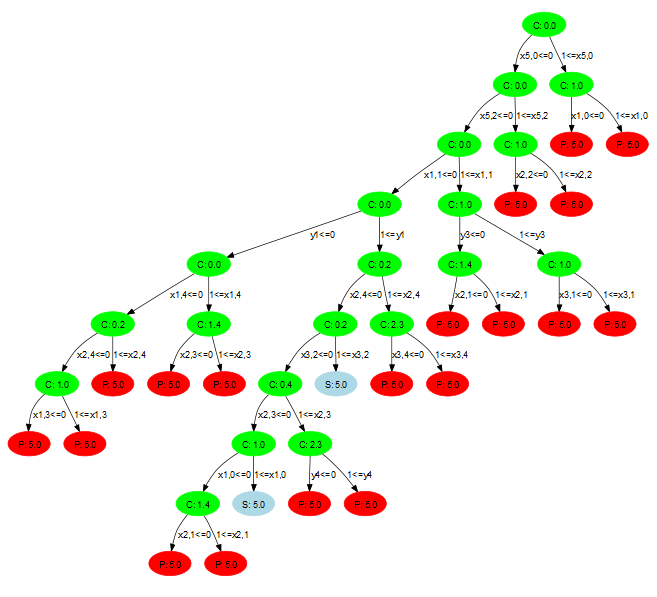
\includegraphics[bb=0 0 815 496,scale=0.50]{img/bpp_tree1.png}
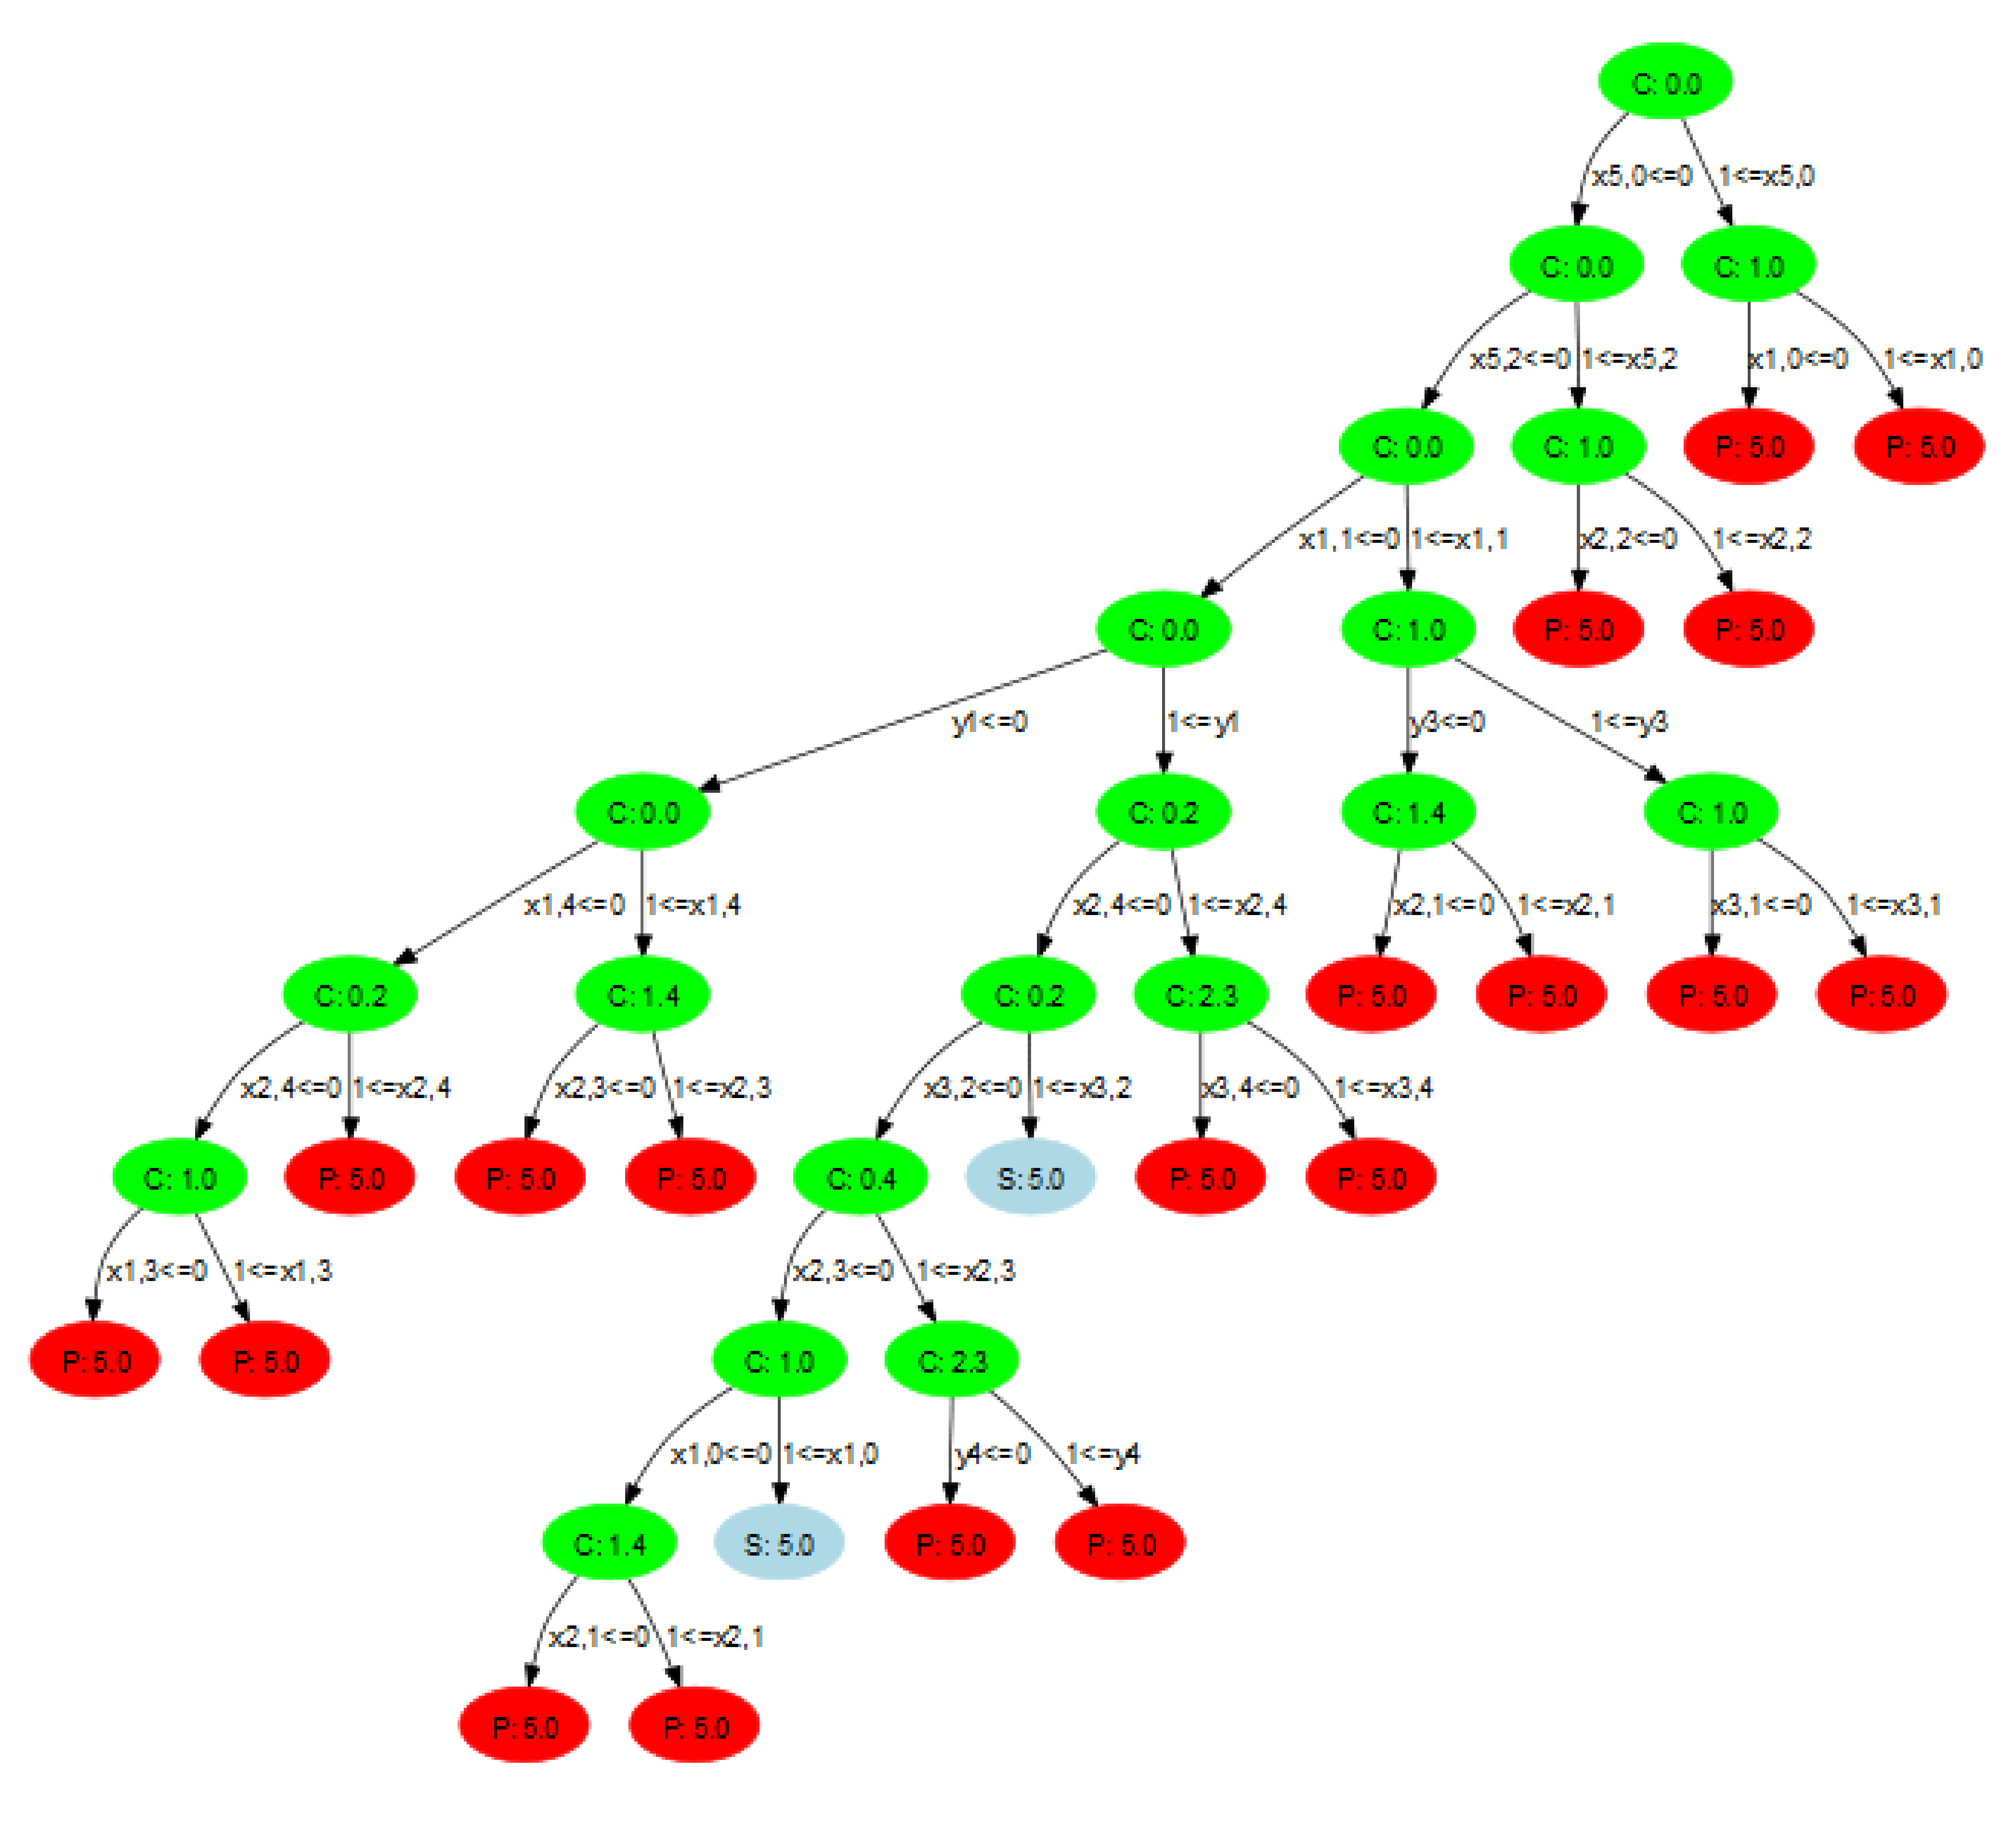
\includegraphics[scale=0.16]{img/bpp_tree1.eps}
\end{center}
\caption{Branch-and-bound tree for bin packing problem instance.} \label{fig:bpp_tree1}
\end{figure}

\subsection{Adding Customised Branching} \label{sbs:branch}
\begin{sloppypar}In \sbsref{sbs:callbacks} we explained the modifications made to \ac{DIP} and how a simple variable branch would be implemented.
The \ac{DIP} function \lstinline{chooseBranchSet} calls Dippy's \lstinline{branch_method} at fractional nodes.
The function \lstinline{branch_method} has two inputs supplied by \ac{DIP}:
\begin{enumerate}
\item \lstinline{prob} -- the \lstinline{DipProblem} being solved;
\item \lstinline{sol} -- an indexable object representing the solution at the current node.
\end{enumerate}
We define \lstinline{branch_method} using these inputs and the same PuLP structures used to defined the model, allowing Dippy to access the variables from the original formulation and eliminating any need for complicated indexing.\end{sloppypar}

We can explore custom branching rules that leverage constraints to reduce the symmetry in the solution space of the bin packing problem.
Inefficiencies arise from solvers considering multiple equivalent solutions that have identical objective function values and differ only in the subset of the identical bins used.
One way to address this is to add a constraint that determines the order in which the bins can be considered:
\[ y_i \geq y_{i+1}, i = 1, \ldots, m-1 \]
\lstinputlisting[firstnumber=61,linerange=61-62]{../../examples/Dippy/bpp/bin_pack_func.py}
This change results in a smaller branch-and-bound tree (see figure \ref{fig:bpp_tree2}) that provides the same solution but with bin 0 used in place of bin 3, i.e., a symmetric solution, but with the bins now used ``in order''.
\begin{figure}[htp]
\begin{center}
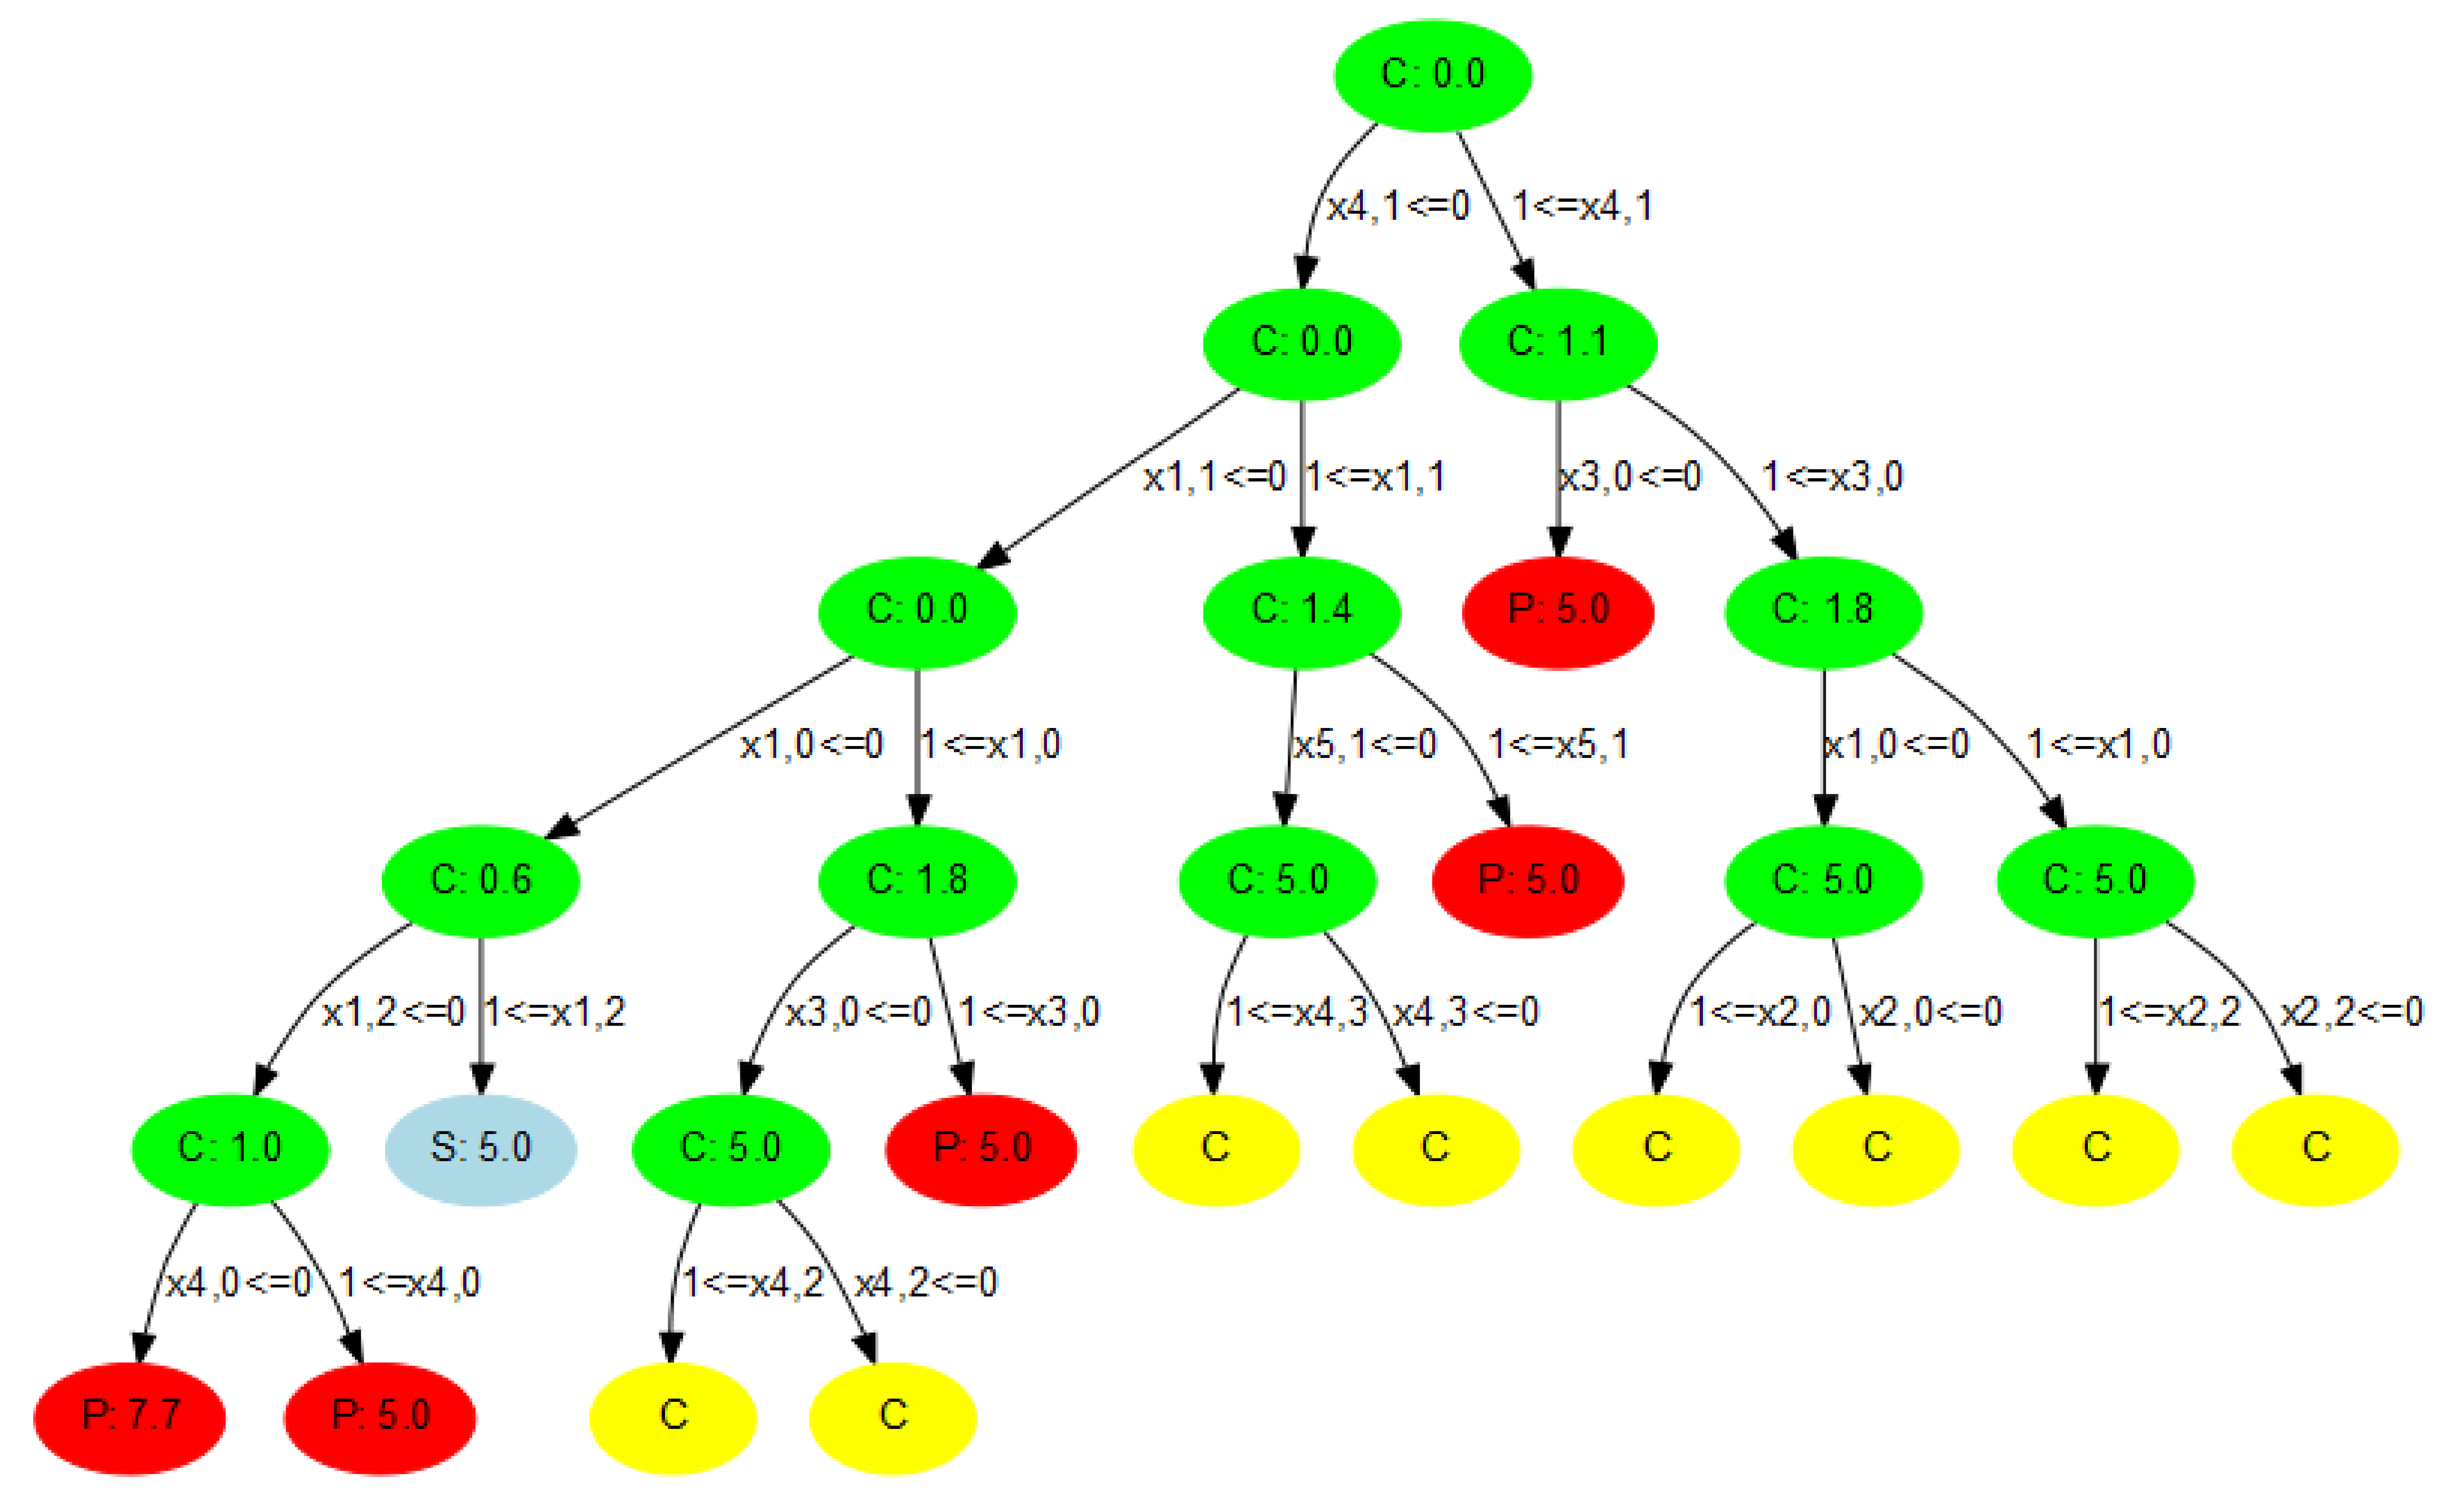
\includegraphics[scale=0.11]{img/bpp_tree2.eps}
\end{center}
\caption{Branch-and-bound tree for bin packing problem instance with anti-symmetry constraints.} \label{fig:bpp_tree2}
\end{figure}

These ordering constraints also introduce the opportunity to implement an effective branch on the number of facilities:

If $\displaystyle\sum_{i=1}^m y_i = \alpha \notin \mathbb{Z}$, then:
\vspace*{-6pt}
\begin{center}
\begin{tabular}{l|l}
the branch down restricts & the branch up restricts \\
$\displaystyle\sum_{i=1}^m y_i \leq \lfloor \alpha \rfloor$ &
$\displaystyle\sum_{i=1}^m y_i \geq \lceil \alpha \rceil$ \\
and the ordering means that & and the ordering means that \\
$y_i = 0, i = \lceil \alpha \rceil, \ldots, m$ &
$y_i = 1, i = 1, \ldots, \lceil \alpha \rceil$
\end{tabular}
\end{center}

\begin{sloppypar}We can implement this branch in Dippy by writing a definition for the \lstinline{branch_method}.\end{sloppypar}
\lstinputlisting[firstnumber=73,linerange={73-75,82-83}]{../../examples/Dippy/bpp/bin_pack_func.py}
\lstinputlisting[firstnumber=182,linerange={182-188,190-193,195-201,203-204,206-207}]{../../examples/Dippy/bpp/bin_pack_func.py}

The advanced branching decreases the size of the branch-and-bound tree further (see figure \ref{fig:bpp_tree3}) and provides another symmetric solution with the bins used in order.
\begin{figure}[htp]
\begin{center}
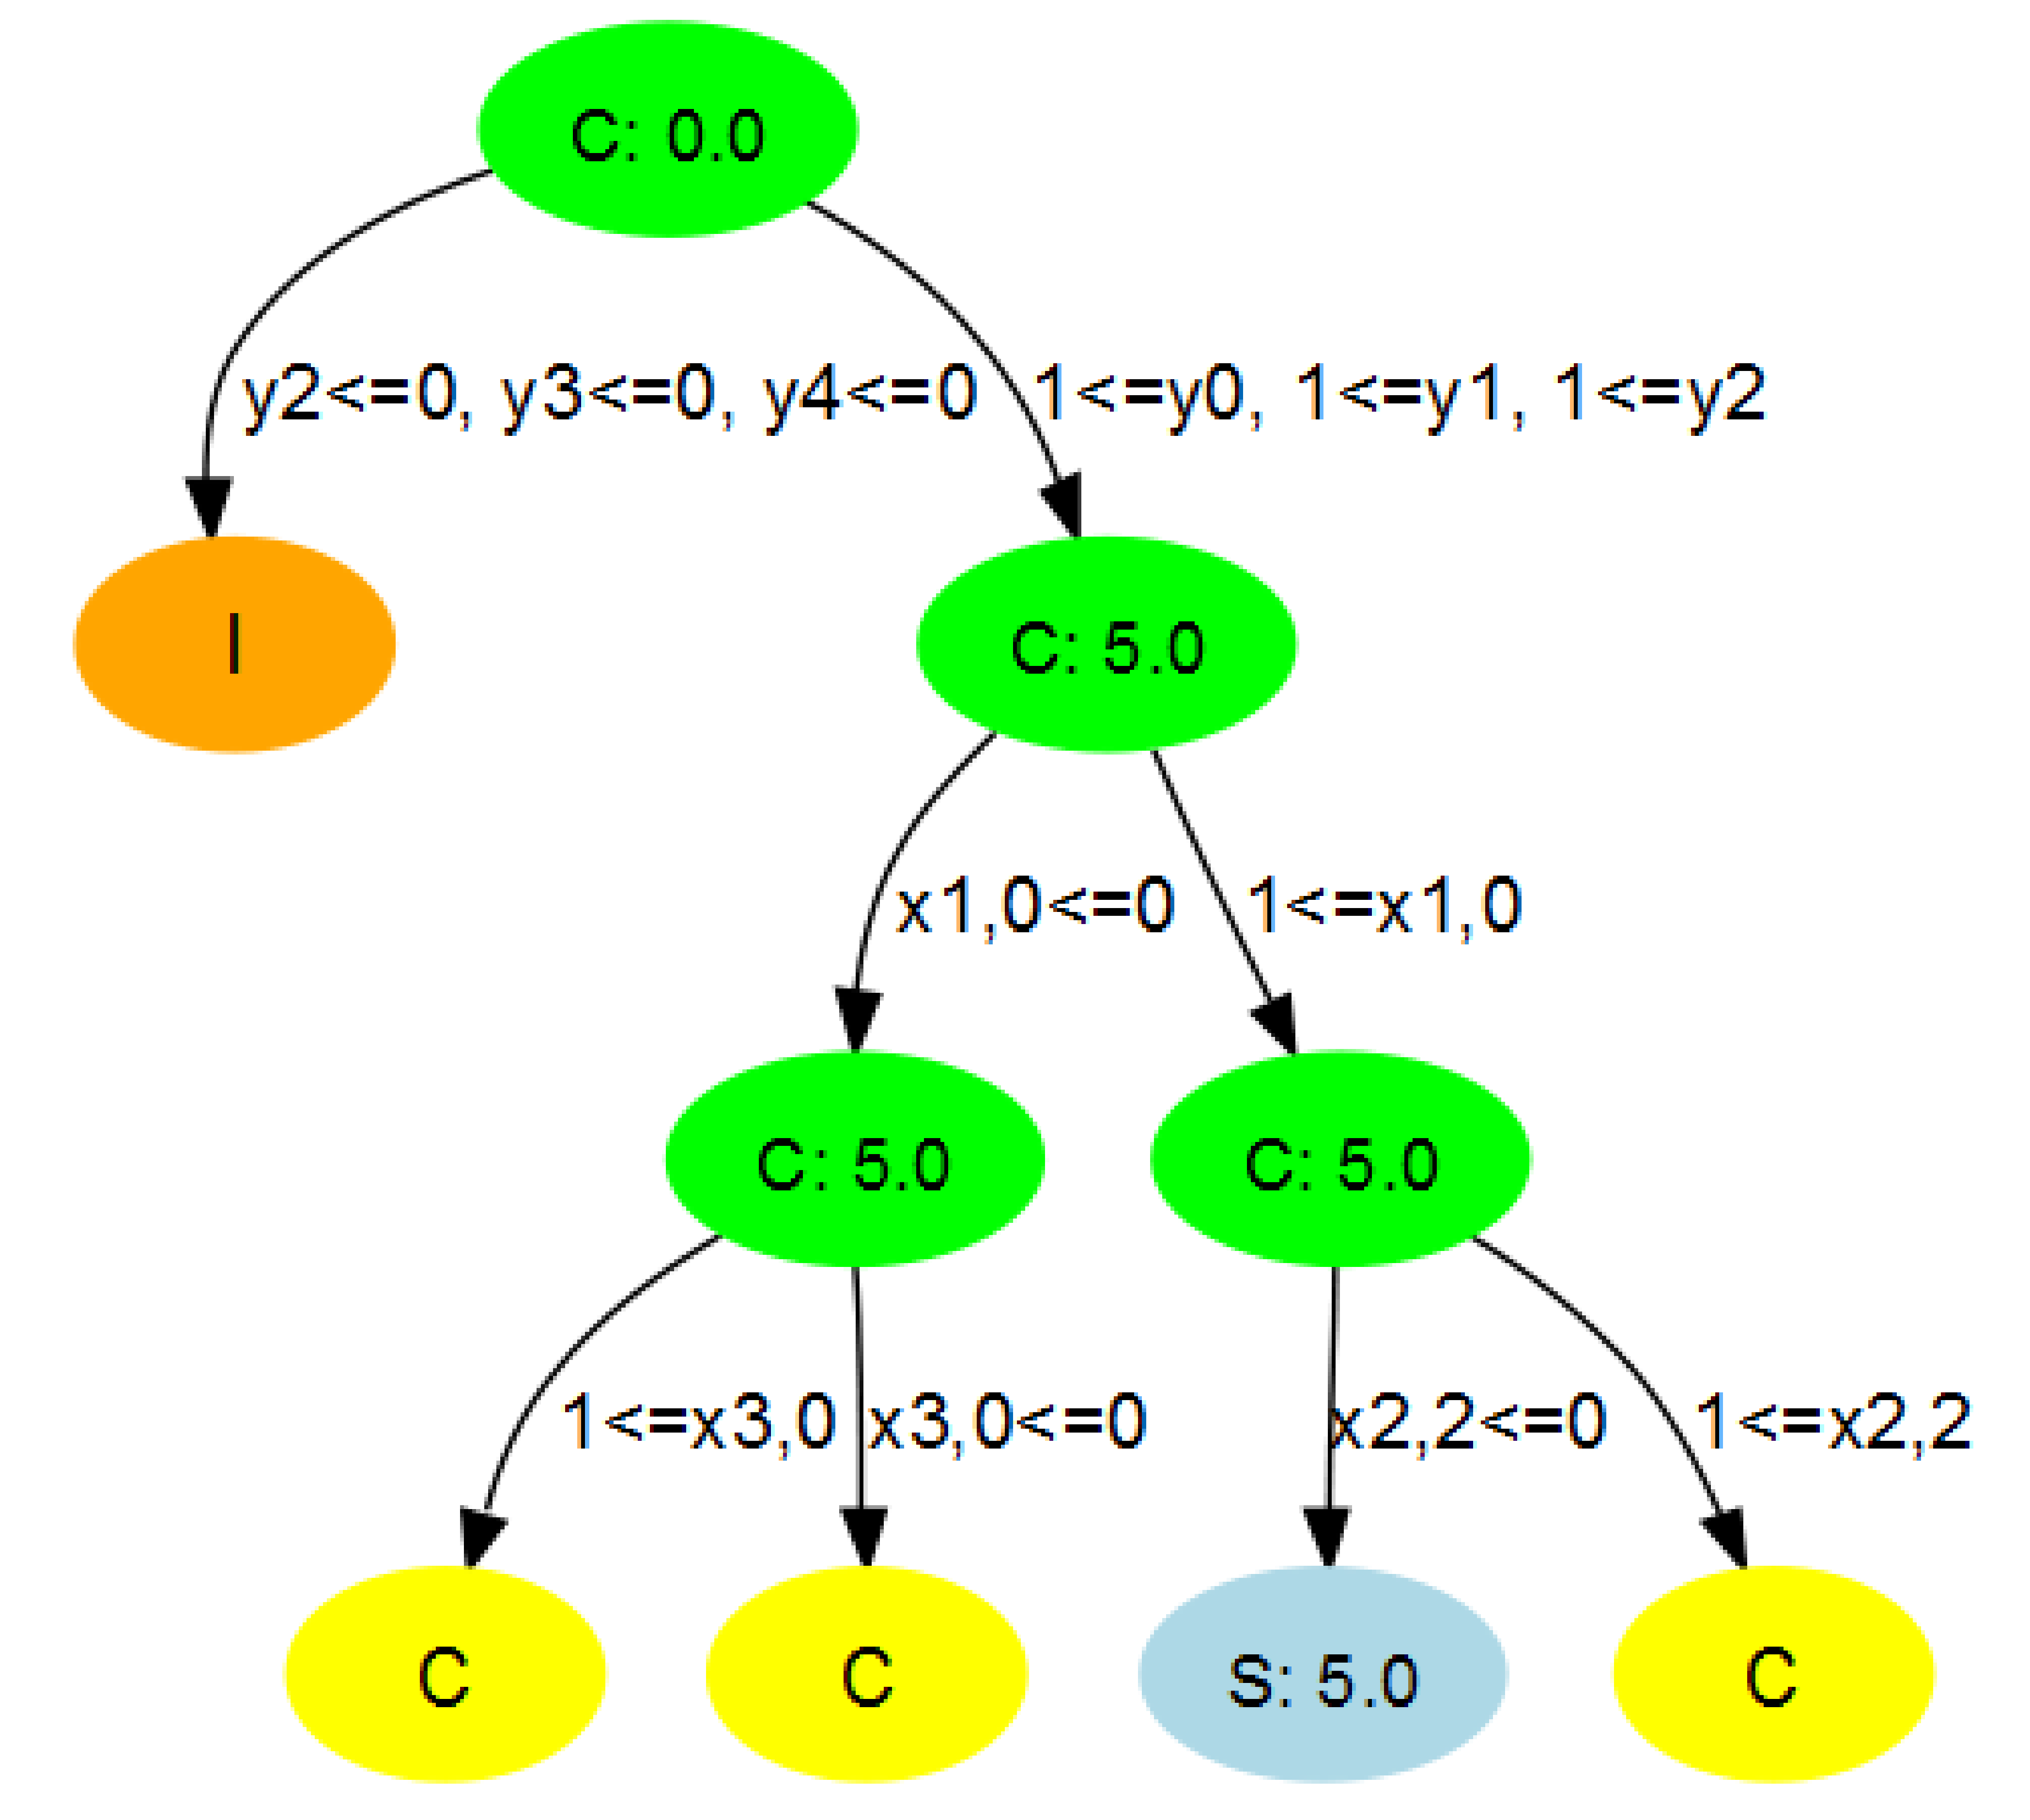
\includegraphics[scale=0.08]{img/bpp_tree3.eps}
\end{center}
\caption{Branch-and-bound tree for bin packing problem instance with anti-symmetry constraints and advanced branching.} \label{fig:bpp_tree3}
\end{figure}


\subsection{Adding Customised Cut Generation} \label{sbs:cuts}
To add user-defined cuts in Dippy, we first define a new procedure for generating cuts and (if necessary) a procedure for determining a feasible solution. Within Dippy, this requires two new functions, \texttt{generate\_cuts} and (if necessary) \texttt{is\_solution\_feasible}. Both these functions have the same inputs as \texttt{branch\_method} (described in \scnref{scn:branch}):
\begin{enumerate}
\item \texttt{prob} -- the \texttt{DipProblem} being solved;
\item \texttt{sol} -- an indexable object representing the solution at the current node.
\end{enumerate}
If a solution is determined not to be feasible either by \ac{DIP} (e.g., if the integer variables don't have integer values) or by \texttt{is\_solution\_feasible}, then cuts are generated (both by \texttt{generate\_cuts} and, if being used, the \ac{CGL}). Different problems benefit from different approaches to cuts as we demonstrate throughout this section. As in \scnref{scn:branch}, Python's scoping rules allow us to easily access the solution values of variables in our problem.

\subsection{Customised Cut Generation for the Capacitated Facility Location problem} \label{sbs:fac_cuts}

Marchand and Wolsey \cite{agg_mir2001} define many types of cuts for \ac{MILP} problems. One of these is the \textit{weighted inequality}. For each facility location $i$ and some subset $S_i (\subseteq 1, \ldots, n)$ of the products we can calculate
\[ \mu_i = W - \sum_{j \in S_i} w_j x_{ij} \]
and use it to generate a weighted inequality
\[ \sum_{j \in S_i} w_j x_{ij} + \sum_{j \notin S_i} (w_j - \mu_i)^+ x_{ij} \leq W - \mu _i \]
which forms a valid inequality for the facility location problem.

To get the subsets $S_i$ for each location from a fractional solution to the facility location problem we have assigned items to locations in a greedy way depending on their $x_{ij}$ values. Once the subsets are determined, we generate a set of weighted inequality cuts.

For brevity we have omitted the generation of $S_i$, but have shown how to build the set of cuts. Again, note that Python's scoping rules allow us to easily access the solution values of variables in our problem.
\lstinputlisting[firstnumber=70,linerange=70-72]{C:/COIN/Dippy/examples/facility.py}
$\vdots$
\lstinputlisting[firstnumber=102,linerange=102-115]{C:/COIN/Dippy/examples/facility.py}

The effect of the weighted inequality cuts is shown in \scnref{scn:concl}.

\subsection{Customised Cut Generation for the Travelling Salesperson problem}

To add user-defined cuts for the \ac{TSP} in Dippy, we define a new procedure for generating cuts (as in \sbsref{sbs:fac_cuts}). For the \ac{TSP} (see \sbsref{sbs:tsp}) we generate cuts to eliminate subtours. In addition, as subtour elimination is not enforced by the original formulation (see \sbsref{sbs:tsp}), we also define \texttt{is\_solution\_feasible} to make sure a feasible solution contains no subtours.

The function for generating subtour elimination cuts finds all subtours in the current solution using the function \texttt{get\_subtour} (omitted here for brevity, \\ \texttt{get\_subtour} finds a subtour from a given node in \texttt{sol}) and adds a cut to eliminate them:
\lstinputlisting[firstnumber=55,linerange=55-75]{C:/COIN/Dippy/examples/tsp.py}

The \texttt{get\_subtour} function can also be used to check if a solution contains any subtours (hence is infeasible):
\lstinputlisting[firstnumber=77,linerange=77-84]{C:/COIN/Dippy/examples/tsp.py}

\Figref{fig:tsp_prob} shows an example \ac{TSP} problem. \Figref{fig:tsp_cuts1} shows the subtours present in the initial solution. After \texttt{is\_solution\_feasible} identifies that there are subtours present in the solution, they are eliminated by cuts created in \\ \texttt{generate\_cuts}. \Figref{fig:tsp_cuts2} shows subtours present in a later solution that are similarly eliminated. After eliminating the necessary subtours, the optimal tour is found -- see \figref{fig:tsp_soln}.
\begin{figure}[ht]
\begin{raggedright}
\begin{tabular}{@{}l@{\ }l}
\subfigure[City locations for the \ac{TSP} example]{
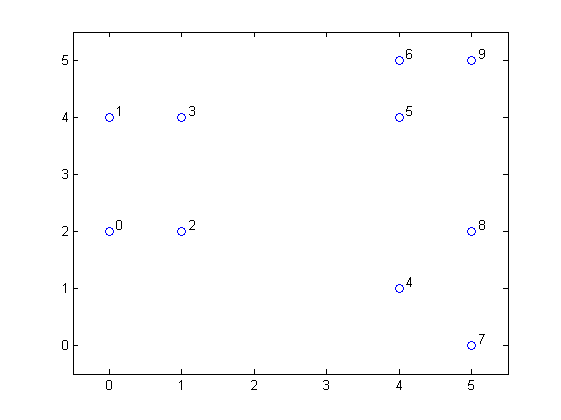
\includegraphics[bb=0 0 561 420,scale=0.37]{tsp_prob.png}
\label{fig:tsp_prob}} &
\subfigure[Subtours from the initial solution to the \ac{TSP} example]{
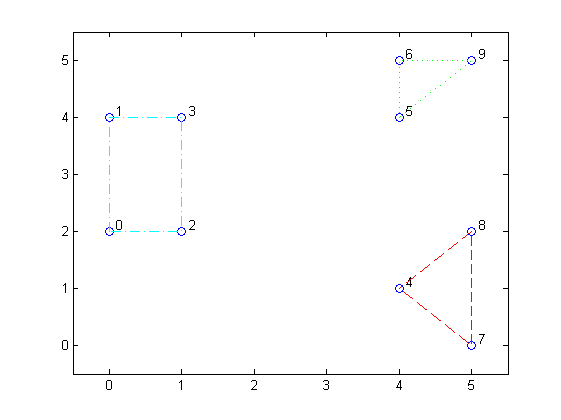
\includegraphics[bb=0 0 561 420,scale=0.37]{tsp_cuts1.png}
\label{fig:tsp_cuts1}}\\
\subfigure[Subtour from a later solution to the \ac{TSP} example]{
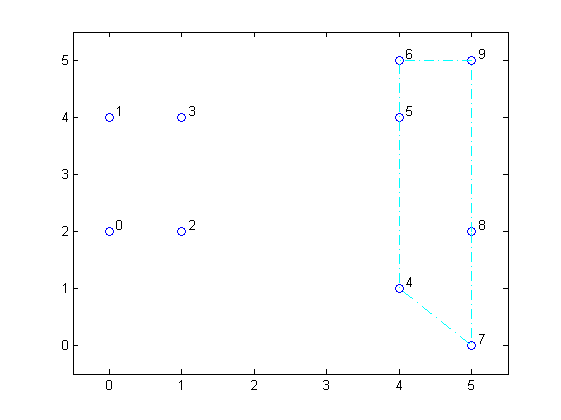
\includegraphics[bb=0 0 561 420,scale=0.37]{tsp_cuts2.png}
\label{fig:tsp_cuts2}} &
\subfigure[Final solution to the \ac{TSP} example]{
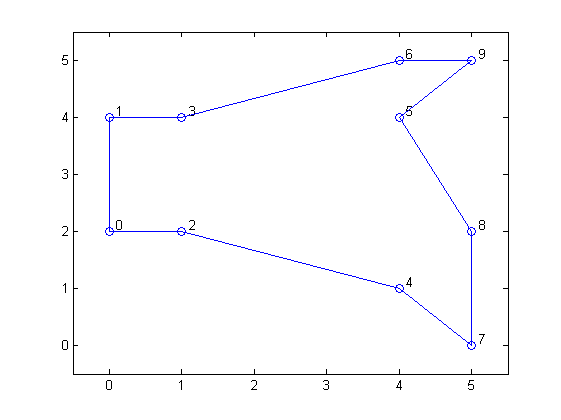
\includegraphics[bb=0 0 561 420,scale=0.37]{tsp_soln.png}
\label{fig:tsp_soln}}
\end{tabular}
\end{raggedright}
\caption{Cuts from an example \ac{TSP}} \label{fig:tsp}
\end{figure}

\begin{comment}
\subsection{Customised Cut Generation for the Wedding Planner problem} \label{sbs:wed_cuts}
\end{comment}

\subsection{Adding Customised Column Generation} \label{sbs:column}
Using Dippy it is easy to transform a problem into a form that can be solved by either branch and cut or branch, price and cut. Branch, price and cut decomposes a problem into a master problem and a number of distinct subproblems. We can identify subproblems using the \texttt{relaxation} member of the \texttt{DipProblem} class (remember the constraints restricting how patterns can be cut in \sbsref{sbs:sponge}). Once the subproblems have been identified, then they can either be ignored (when using branch and cut -- the default method for \ac{DIP}) or utilised (when using branch, price and cut -- specified by turning on the \texttt{doPriceCut} option).

\vfill
\newpage

In branch, price and cut, the original problem is decomposed into a master problem and multiple subproblems:
\begin{equation}
\begin{array}{rr@{\ }r@{\ }r@{\ }r@{\ }l}
             \min & c_1^\top x_1 & + \ c_2^\top x_2 & + \ \cdots & + \ c_k^\top x_k \\
\text{subject to} & A_1 x_1      & + \ A_2 x_2      & + \ \cdots & + \ A_k x_k      & = b \\
                  &              &   F_2 x_2      &          &                & = f_2 \\
                  &              &                &  \ddots  &                & \ \ \vdots \\
                  &              &                &          &   F_k x_k      & = f_k \\
                  & x_1 \in \mathbb{Z}^{+}_{n_1} &, x_2 \in \mathbb{Z}^{+}_{n_2}&, \ldots, x_k & \in \mathbb{Z}^{+}_{n_k} \quad
\end{array}
\label{eqn:decomp}
\end{equation}

Then, given a subset of extreme points for each subproblem, the \textit{restricted} master problem (RMP) finds an optimal solution and corresponding duals ($\pi$, $\gamma_1, \ldots, \gamma_k$):
\begin{equation}
\begin{array}{rr@{\ }r@{\ }r@{\ }r@{\ }ll}
             \min & c_1^\top x_1 & + \displaystyle\sum_{l_2=1}^{L_2} \left(c_2^\top y^2_{l_2} \right) \lambda^2_{l_2} & + \ \cdots & + \displaystyle\sum_{l_k=1}^{L_k} \left(c_k^\top y^k_{l_k} \right) \lambda^k_{l_k} \\
\text{subject to} & A_1 x_1      & + \displaystyle\sum_{l_2=1}^{L_2} \left(A_2 y^2_{l_2} \right) \lambda^2_{l_2} & + \ \cdots & + \displaystyle\sum_{l_k=1}^{L_k} \left( A_k y^k_{l_k} \right) \lambda^k_{l_k}      & = b & : \pi \\
                  &              &   \displaystyle\sum_{l_2=1}^{L_2} \lambda^2_{l_2}      &          &                & = 1 & : \gamma_1 \\
                  &              &                &  \ddots  &                & \ \ \vdots \\
                  &              &                &          &   \displaystyle\sum_{l_k=1}^{L_k} \lambda^k_{l_k}      & = 1 & : \gamma_k \\
                  &          x_1 & \in \mathbb{Z}^{+}_{n_1}, \lambda^2 \in \{0, 1\}_{L_2}, & \ldots, \lambda^k & \in \{0, 1\}_{L_k} \hspace{1.25cm} &
\end{array}
\label{eqn:rmp}
\end{equation}

New extreme points (columns for the RMP) are found by solving the subproblems ${\cal S}_j, j = 1, \ldots, k$ with the objective of minimising the reduced cost of a column in the RMP:
\begin{equation}
\begin{array}{rrl}
{\cal S}_j: \min & (c_j - \pi^\top A_j)^\top x_j + \gamma_j \\
\text{subject to} & F_j x_j      & = f_j \\
                  & x_j \in \mathbb{Z}^{+}_{n_j}
\end{array}
\label{eqn:subprob}
\end{equation}
If the objective value of ${\cal S}_j$ is $< 0$, then the column will improve the objective value of the RMP and is added.

The subproblems can either be solved using the default \ac{MILP} solver (Cbc) or a customised solver. A customised solver can be defined by the \texttt{relaxed\_solver} function. This function has 4 inputs:
\begin{enumerate}
\item \texttt{prob} -- the \texttt{DipProblem} being solved;
\item \texttt{index} -- the index $j$ of the subproblem being solved;
\item \texttt{redCosts} -- $c_j - \pi^\top A_j$, the reduced costs for the $x_j$ variables;
\item \texttt{convexDual} -- $\gamma_j$, the dual value for the convexity constraint for this subproblem.
\end{enumerate}
In addition to subproblem solutions using dual values, initial columns for subproblems can also be generated either automatically using Cbc or using a customised approach. A customised approach to initial variable generation can be defined by the \texttt{init\_vars} function. This function has only 1 input, \texttt{prob}, the \texttt{DipProblem} being solved.

\subsection{Customised Column Generation for the Capacitated Facility Location problem} \label{sbs:fac_cols}

Starting from the original capacitated facility location problem (see \sbsref{sbs:facility}), we can define subproblems for each facility location that define the capacity constraints at that location:
\lstinputlisting[firstnumber=35,linerange=35-44]{C:/COIN/Dippy/examples/facility_decomp.py}

All remaining constraints (the assignment constraints - ensuring each product is assigned to a facility) form the master problem when using branch, price and cut. To use branch, price and cut we turn on the \texttt{doPricCut} option:
\lstinputlisting[firstnumber=162,linerange=162-166]{C:/COIN/Dippy/examples/facility_decomp.py}

Note that symmetry is also present in the decomposed problem, so we add the ordering constraints to the RMP (see \sbsref{sbs:fac_brch}):
\lstinputlisting[firstnumber=46,linerange=46-49]{C:/COIN/Dippy/examples/facility_decomp.py}

In branch, price and cut, the RMP requires 10.39s of CPU times and creates a tree with 27 nodes (compared with 0.28s and 76 nodes for the original branch and cut approach with ordering constraints). Note that the \texttt{generateInitVars} option uses Cbc by default to find initial columns for the RMP and then Cbc is also used (by default) to solve the subproblems that generate facilities at locations along with products produced at that facility. However, we may be able to speed up the overall solution process by providing our own approaches to solving the pricing subproblems and generating initial variables.

In the pricing subproblem, we are looking to assign products to a facility in order to provide negative reduced cost. Producing a product at a facility provides the reduced cost of $x_{ij}$ (\texttt{assign\_vars[(i, j)]}), but will decrease the wasted capacity and hence reduce the contribution of the reduced cost of $w_i$ (\texttt{waste\_vars[i]}). Here, we calculate the total contribution to reduced cost of adding an item (= reduced cost of $x_{ij} -$ reduced cost of $w_i \times r_j$) and then calculate an items efficiency by dividing this contribution by its weight. Then, we build a minimum reduced cost facility by using a greedy algorithm to choose items in order of best efficiency. Since we can access the problem data, variables and their reduced cost, this is straightforward to implement in Dippy:
\lstinputlisting[firstnumber=69,linerange=69-105]{C:/COIN/Dippy/examples/facility_decomp.py}

Adding this customised solver reduces the solution time to 1.61s of CPU time and the search tree to 7 nodes.

To generate initial facilities (complete with assigned products) we implemented two approaches. The first approach used a first-fit approach and considered the products in order of decreasing requirement:
\lstinputlisting[firstnumber=107,linerange=107-138]{C:/COIN/Dippy/examples/facility_decomp.py}

The second approach simply assigned one product to each facility:
\lstinputlisting[firstnumber=140,linerange=140-153]{C:/COIN/Dippy/examples/facility_decomp.py}

\newpage

Using Dippy we can define both approaches at once and then define which one to use by setting the \texttt{init\_vars} method:
\lstinputlisting[firstnumber=155,linerange=155-156]{C:/COIN/Dippy/examples/facility_decomp.py}

The effects of column generation, included a customised subproblem solver and initial variable generator are shown in \scnref{scn:concl}.

\subsection{Customised Column Generation for the Cutting Stock problem} \label{sbs:cut_cols}

For the Sponge Roll Production problem (see \sbsref{sbs:sponge}), the subproblem consists of the cutting pattern constraint:
\lstinputlisting[firstnumber=55,linerange=55-59]{C:/COIN/Dippy/examples/cutting_stock.py}

To generate cutting patterns with negative reduced cost in the customised \texttt{relaxed\_solver} function, we first set ``profit'' coefficients to be $-$ reduced cost and ``size'' coefficients to be the length of the required items:
\lstinputlisting[firstnumber=62,linerange=62-68]{C:/COIN/Dippy/examples/cutting_stock.py}

Then, we use \ac{DP} to find a maximum profit knapsack. The \ac{DP} recursion is:
\[\begin{array}{rcl}
I &=& \text{set of possible items to include}; \\
W &=& \text{capacity of knapsack}; \\
w_i &=& \text{``size'' of item } i; \\
p_i &=& \text{``profit'' of including item} i; \\
V(I, W) &=& \text{maximum profit when considering items from $I$} \\
& &\text{for inclusion in a knapsack of capacity $W$} \\
V(\emptyset, W) &=& 0 \\
V(I, 0) &=& 0 \\
V(I, W) &=& \max\big[\underset{\text{\begin{tabular}{c}don't include any \\[-3pt] item, consider \\[-3pt] smaller knapsack \end{tabular}}}{\underbrace{V(I, W - 1)}}, \max_{i \in I} \underset{\text{include item $i$}}{\underbrace{p_i + V(I, W - w_i)}} \big].
\end{array}\]

\newpage

The \texttt{kp} function implements the \ac{DP} recursion:
\lstinputlisting[firstnumber=97,linerange=97-122]{C:/COIN/Dippy/examples/cutting_stock.py}

The customised \texttt{relaxed\_solver} function calls \texttt{kp} to find the maximum profit (= most negative reduced cost) cutting pattern:
\lstinputlisting[firstnumber=70,linerange=70-70]{C:/COIN/Dippy/examples/cutting_stock.py}
checks it is valid and adds it to the restricted master problem if the total reduced cost is negative (cutting pattern reduced cost + pattern use reduced cost $-$ convexity constraint dual $< 0$).
\lstinputlisting[firstnumber=79,linerange=79-93]{C:/COIN/Dippy/examples/cutting_stock.py}

The effect of the customised subproblem solver is a reduction from 33.31s to 28.30s of CPU time and 175 to 131 nodes.

\begin{comment}
\subsection{Customised Column Generation for the Wedding Planner problem} \label{sbs:wed_cols}
\end{comment}

\newpage\subsection{Adding Customised Heuristics} \label{sbs:heuristics}
To add user-defined heuristics in Dippy, we first define a new procedure for node heuristics, \texttt{heuristics}. This function has three inputs:
\begin{enumerate}
\item \texttt{prob} -- the \texttt{DipProblem} being solved;
\item \texttt{xhat} -- an indexable object representing the fraction solution at the current node;
\item \texttt{cost} -- the objective coefficients of the variables.
\end{enumerate}
Multiple heuristics can be executed and all heuristic solutions can be returned to \ac{DIP}. Different problems benefit from different heuristic approaches and a heuristic that solves the original problem may not be as useful when a fractional solution is available. We show how solve a heuristic for the overall problem and also how to implement a heuristic for fractional solutions. As in \scnref{scn:branch}, Python's scoping rules allow us to easily access the solution values of variables in our problem.

\subsection{Customised Heuristics for the Capacitated Facility Location problem} \label{sbs:fac_heur}

An initial allocation of production to locations can be found heuristically using the same first-fit heuristic that provided initial solutions for the column generation approach (see \sbsref{sbs:fac_cols}). The first-fit heuristic iterates through the items requiring production and the facility locations allocating production at the first facility that has sufficient capacity to produce the item.
\lstinputlisting[firstnumber=116,linerange=116-127]{C:/COIN/Dippy/examples/facility.py}

\vfill
\newpage
\lstinputlisting[firstnumber=129,linerange=129-144]{C:/COIN/Dippy/examples/facility.py}

The first-fit heuristic can then be used to provide an initial, feasible solution at the root node within the customised \texttt{heuristics} function (see lines 215-220):
\lstinputlisting[firstnumber=211,linerange=211-230]{C:/COIN/Dippy/examples/facility.py}

Running the first-fit heuristic before starting the branching process increases the solution time from 1.17s to 1.48s of CPU time and the number of nodes in the search tree from 375 nodes to 399 nodes.

\newpage

At each node in the branch-and-bound tree, the fractional solution (provided by \texttt{xhat}) gives an indication of the best allocation of production, albeit fractional. One heuristic approach to ``fixing'' the fractional solution is to consider each allocation (of an item's production to a facility) in order of decreasing fractionality and use a first-fit approach:
\lstinputlisting[firstnumber=146,linerange=146-192]{C:/COIN/Dippy/examples/facility.py}
\newpage
\lstinputlisting[firstnumber=194,linerange=194-209]{C:/COIN/Dippy/examples/facility.py}

The first-fit approach that is guided by fractional values can then be used within the \texttt{heuristics} function (see lines 225-229 in the previous listing) to create integer solutions from fractional solutions at each node.

Adding the first-fit heuristic guided by fractional values increases the solution time further from 1.48s to 1.89s of CPU time and the number of nodes remains at 399.

The reason this heuristic (in fact any heuristic) was not that helpful for this problem is that:
\begin{itemize}
\item the optimal solution is found within the first 10 nodes without any heuristics, so the heuristic only provides an improved upper bound for $< 10$ nodes;
\item the extra overhead of the heuristic at each node increases the solution time and the heuristic affects the search procedure in a way that more nodes are explored.
\end{itemize}

Heuristics generally only help in problems where feasibility is more difficult by providing upper bounds when ``fixing'' fractional solutions. In this problem, the optimal solution is found quickly and the rest of the search tree checks solutions that are symmetric.

In \scnref{scn:concl} we show the effect of the heuristic when symmetry is removed.

\begin{comment}
\subsection{Customised Heuristics for the Wedding Planner problem} \label{sbs:wed_heur}
\end{comment}

\subsection{Combining Techniques} \label{sbs:combine}

\begin{table}[ht]
%\begin{minipage}[c]{\textwidth}
%\begin{small}
\begin{center}
\begin{tabular}[c]{|lll|}
\hline
\textbf{Strategies}																 & \textbf{Time (s)}	& \textbf{Nodes} \\ 
\hline & &\\[-10pt]
Default (branch and cut)                           & 0.26							  & 419 \\
\hline
+ ordering constraints (OC)                        & 0.05 							& 77 \\
+ OC \& advanced branching (AB)                    & 0.01 							& 3 \\
\hline
+ weighted inequalities (WI)                       & 0.34 							& 77 \\
+ WI \& OC                                         & 0.17 							& 20 \\
+ WI \& OC \& AB                                   & 0.06 							& 4 \\
\hline
+ first-fit heuristic (FF) at root node            & 0.28 							& 419 \\
+ FF \& OC                                         & 0.05 							& 77 \\
+ FF \& OC \& AB                                   & 0.01 							& 3 \\
\hline
+ FF \& WI                                         & 0.36 							& 77 \\
+ FF \& WI \& OC                                   & 0.14 							& 17 \\
+ FF \& WI \& OC \& AB                             & 0.05 							& 3 \\
\hline
+ fractional-fit heuristic (RF) at nodes           & 0.28 							& 419 \\
+ RF \& OC                                         & 0.05 							& 77 \\
+ RF \& OC \& AB                                   & 0.01 							& 3 \\
\hline
+ WI \& RF                                         & 0.38 							& 77 \\
+ WI \& RF \& OC                                   & 0.14 							& 17 \\
+ WI \& RF \& OC \& AB                             & 0.05 							& 3 \\
\hline
+ FF \& RF                                         & 0.28 							& 419 \\
+ FF \& RF \& OC                                   & 0.05 							& 77 \\
+ FF \& RF \& OC \& AB                             & 0.01 							& 3 \\
\hline
+ WI \& FF \& RF                                   & 0.38 							& 77 \\
+ WI \& FF \& RF \& OC                             & 0.14 							& 17 \\
+ WI \& FF \& RF \& OC \& AB                       & 0.05 							& 3 \\
\hline
+ column generation (CG)                           & 2.98 							& 37 \\
+ CG \& OC                                         & 2.07 							& 23 \\
+ CG \& OC \& AB                                   & 0.56								& 10 \\
\hline
+ CG \& customised subproblem solver (CS)          & 2.87 							& 37 \\
+ CG \& CS \& OC                                   & 1.95 							& 23 \\
+ CG \& CS \& OC \& AB                             & 0.44 							& 10 \\
\hline
+ CG \& first-fit initial variable generation (FV) & 3.96 							& 45 \\
+ CG \& CS \& FV                                   & 3.72 							& 45 \\
+ CG \& CS \& FV \& OC                             & 1.70 							& 18 \\
+ CG \& CS \& FV \& OC \& AB                       & 0.22 							& 3\\
\hline
+ CG \& one-each initial variable generation (OV)  & 3.40 							& 41 \\
+ CG \& CS \& OV                                   & 3.33 							& 41 \\
+ CG \& CS \& OV \& OC                             & 2.23 							& 24 \\
+ CG \& CS \& OV \& OC \& AB                       & 0.27 							& 3 \\
\hline
\end{tabular} 
\end{center}
%\end{small}
%\end{minipage}
\caption{Experiments for the Capacitated Facility Location Problem} \label{tab:fac_exp}
\end{table}

The techniques and modifications of the solver framework can be combined to improve performance further.
\Tabref{tab:fac_exp} shows that it is possible to quickly and easily test many approaches for a particular problem, including combinations of approaches\footnote{All tests were run using Python 2.7.1 on a Windows~7 machine with an Intel Core~2~Duo T9500@2.60GHz CPU.}.
Looking at the results shows that the heuristics only help when the size of the branch-and-bound tree has been reduced with other approaches, such as ordering constraints and advanced branching.
Approaches for solving this problem that warrant further investigation use column generation, the customised solver and either ordering constraints or the first-fit heuristic to generate initial variables.
Tests with different data showed that the solution time for branch-price-and-cut doesn't increase with problem size as quickly as for branch-and-cut, so the column generation approaches are worth considering for larger problems.


\section{Performance and Conclusions} \label{scn:concl}
In this paper we have presented Dippy, a simplified interface to advanced \acl{MILP} techniques.The main motivation for the development of Dippy was to alleviate obstacles to experimentation with and customisation of advanced \ac{MILP} frameworks. We have shown using case studies that Dippy is relatively simple to experiment with and customise. Using Dippy we have improved the solution performance of:
\begin{itemize}
\item The Coke Supply Chain problem by adding advanced branching, reducing the solution CPU time from 1.09s to 0.62s of CPU time and branch-and-bound tree from 201 nodes to 76 nodes;
\item The Travelling Salesperson problem by adding subtour elimination cuts to create an optimal tour without adding all subtour elimination constraints;
\item The Cutting Stock problem by adding a customised subproblem solver, reducing the solution CPU time from 33.31s to 28.30s and the branch-and-bound tree from 175 to 131 nodes.
\end{itemize}
We have experimented with advanced branching, customised cuts, customised column generation and heuristics for the Capacitated Facility Location problem and Dippy enables us to quickly obtain a table of experimental results, see \tabref{tab:fac_exp}.
\begin{table}[htp]
\begin{minipage}[l]{\textwidth}
\begin{small}
\begin{tabular}{|lll|}
\hline
\textbf{Strategies} & \textbf{Time (s)}   & \textbf{Nodes} \\ \hline & &\\[-10pt]
Default (branch and cut)                           & 1.17 & 375 \\
+ ordering constraints (OC)                        & 0.28 & 76 \\
+ OC \& advanced branching (AB)                    & 0.05 & 3 \\
+ weighted inequalities (WI)                       & 1.11 & 43 \\
+ OC \& WI                                         & 0.61 & 17 \\
+ OC \& AB \& WI                                   & 0.27 & 4 \\
+ first-fit heuristic (FF) at root node            & 1.52 & 399 \\
+ OC \& FF                                         & 0.30 & 76 \\
+ OC \& AB \& FF                                   & 0.02 & 3 \\
+ WI \& FF                                         & 1.17 & 43 \\
+ OC \& WI \& FF                                   & 0.77 & 19 \\
+ OC \& AB \& WI \& FF                             & 0.20 & 3 \\
+ fractional-fit heuristic (RF) at nodes           & 1.70 & 399 \\
+ OC \& RF                                         & 0.36 & 76 \\
+ OC \& AB \& RF                                   & 0.02 & 3 \\
+ WI \& RF                                         & 1.23 & 43 \\
+ OC \& WI \& RF                                   & 0.80 & 19 \\
+ OC \& AB \& WI \& RF                             & 0.20 & 3 \\
+ FF \& RF                                         & 1.70 & 399 \\
+ OC \& FF \& RF                                   & 0.34 & 76 \\
+ OC \& AB \& FF \& RF                             & 0.02 & 3 \\
+ WI \& FF \& RF                                   & 1.25 & 43 \\
+ OC \& WI \& FF \& RF                             & 0.80 & 19 \\
+ OC \& AB \& WI \& FF \& RF                       & 0.22 & 3 \\
+ column generation (CG)                           & 13.48 & 33 \\
+ CG \& OC                                         & 10.27 & 27 \\
+ CG \& OC \& AB                                   & \multicolumn{2}{l|}{AB fails in Phase 1 with CG. \footnote{If there are insufficient columns to build a feasible solution, i.e., in Phase 1, then our advanced branching introduces constraints that cause infeasibility. However, with columns that provide a feasible solution or our customised subproblem solver, our advanced branching does not cause infeasibility.}}\\
+ CG \& customised subproblem solver (CS)          & 7.59  & 35 \\
+ CG \& CS \& OC                                   & 1.63  & 7 \\
+ CG \& CS \& OC \& AB                             & 1.66  & 8 \\
+ CG \& first-fit initial variable generation (FV) & 11.92 & 31 \\
+ CG \& CS \& FV                                   & 0.33  & 1 \\
+ CG \& CS \& FV \& OC                             & 7.59  & 17 \\
+ CG \& CS \& FV \& OC \& AB                       & 1.23  & 3\\
+ CG \& one-each initial variable generation (OV)  & 10.23 & 25 \\
+ CG \& CS \& OV                                   & 15.61 & 57 \\
+ CG \& CS \& OV \& OC                             & 5.30  & 21 \\
+ CG \& CS \& OV \& OC \& AB                       & 0.91  & 3 \\
\hline
\end{tabular} 
\end{small}
\end{minipage}
\caption{Experiments for the Capacitated Facility Location Problem} \label{tab:fac_exp}
\end{table}

\Tabref{tab:fac_exp} shows that it is possible to quickly and easily test many approaches for a particular problem, including combinations of approaches. Looking at the results shows that the heuristics (from \scnref{scn:heuristics}) only help when the size of the branch-and-bound tree has been reduced with other approaches, e.g., ordering constraints and advanced branching. Other good approaches to test further for the Capacitated Facility Location problem use column generation, the customised solver and either ordering constraints or the first-fit heuristic to generate initial variables. As we shall see later in this section, the solution time for branch, price and cut doesn't increase with problem size as quickly as for branch and cut, so the column generation approaches are worth considering for larger problems.

The one case study not utilised earlier in this paper is the Wedding Planner problem. We used this case study to compare the branch, price and cut framework in \ac{DIP} to the leading open source branch and cut framework, Cbc. Since \ac{DIP}, hence Dippy, doesn't require a problem to be explicitly formulated as a Dantzig-Wolfe decomposition, the change from \ac{DIP} to Cbc is trivial. The only differences are that:
\begin{enumerate}
\item A \texttt{LpProblem} is created instead of a \texttt{DipProblem};
\item No \texttt{.relaxation} statements are used;
\item The \texttt{LpProblem.solve} method uses Cbc to solve the problem.
\end{enumerate}

To see if Cbc would perform well solving a column-based approach, we also formulated the a problem equivalent to the restricted master problem from the branch, price and cut approach and a priori generated and added all possible columns. Finally, we developed a customised solver and initial variable generation for the branch, price and cut formulation in \ac{DIP}. We tested these six approaches, i.e.,
\begin{enumerate}
\item Cbc called from PuLP;
\item Cbc called from PuLP using a columnwise formulation and generating all columns a priori;
\item Gurobi called from PuLP;
\item Gurobi called from PuLP using a columnwise formulation and generating all columns a priori;
\item \ac{DIP} called from Dippy using branch, price and cut without customisation;
\item \ac{DIP} called from Dippy using customised branch, cut and price;
\end{enumerate}
on problem instances of increasing size. All tests were run using Python 2.7.1 on A Dell Precision M4300 laptop with Intel Core 2 Duo CPU T9500@2.60GHz chipset and 777MHz, 3.50GB of RAM.  We used Cbc version 2.30.00, Gurobi version 4.0.1, \ac{DIP} version 0.8.7 and Dippy version 1.0.8. In \Tabref{tab:wed_exp} and \figref{fig:compare} we see that:
\begin{itemize}
\item Gurobi is faster for small problems;
\item The symmetry present in the Capacitated Facility Location problem means the solution time of Cbc and Gurobi for the original problem deteriorate quickly;
\item The time taken to solve the columnwise formulation also deteriorates, but at a lesser rate than when using Cbc or Gurobi on the original problem;
\item Gurobi (using the original formulation) and the column generation approach in \ac{DIP} are less predictable than the Cbc approaches, e.g., the solution time drops for both approaches in a couple of places;
\item Both \ac{DIP} and customised \ac{DIP} solution times grow at a lesser rate than any of the Cbc/Gurobi approaches;
\item For large problems, \ac{DIP} becomes the preferred approach.
\end{itemize}
\begin{table}[htp]
\begin{minipage}[l]{\textwidth}
\begin{small}
\begin{tabular}{|l@{\,}|c@{\ }c@{\ }c@{\ }c@{\ }c@{\ }c@{\ }c@{\ }c@{\,}|}
\hline
\textbf{Guest List} & \multicolumn{8}{|c|}{\textbf{Time (s)}} \\
\textbf{A to $\ldots$} & Cbc & \multicolumn{2}{c}{Cbc \& columns} & Gurobi & \multicolumn{2}{c}{Gurobi \& columns} & \ac{DIP} & Customised \\
\textbf{(\# guests)} & & gen vars & solve & & gen vars & solve & & \ac{DIP} \\ \hline & & & & \\[-10pt]
F	(6) &     0.234&     0.032&     0.234&     0.094&     0.016&     0.203&     3.281&     5.594 \\
G	(7) &     0.297&     0.031&     0.594&     0.156&     0.015&     0.532&     3.984&     8.719 \\
H	(8) &     3.375&     0.015&     1.141&     0.313&     0.031&     1.094&    24.078&    22.688 \\
I	(9) &    14.063&     0.031&     2.547&     0.344&     0.031&     2.422&     7.547&    18.360 \\
J	(10)&   17.047 &    0.016 &    5.422 &    0.406 &    0.031 &    5.344 &   35.250 &   33.828  \\
K	(11)&   25.922 &    0.015 &   10.750 &    0.547 &    0.016 &   10.578 &   64.516 &   59.312  \\
L	(12)&  148.938 &    0.031 &   20.125 &    1.547 &    0.016 &   20.156 &   60.687 &   87.157  \\
M	(13)&  396.141 &    0.031 &   37.250 &    1.890 &    0.031 &   37.422 &   80.079 &  114.515  \\
N	(14)&  398.859 &    0.031 &   66.281 &    1.297 &    0.032 &   65.656 &  142.937 &  142.922  \\
O	(15)&  421.985 &    0.031 &  111.703 &    1.734 &    0.031 &  112.765 &  162.390 &  226.797  \\
P	(16)&14768.676 &    0.031 &  184.016 &  387.641 &    0.047 &  184.734 &  311.218 &  226.875  \\
Q	(17)&      -- &    0.047 &  297.344 &  525.688 &    0.047 &  296.406 &  205.968 &  311.797  \\
R	(18)&      -- &    0.047 &  463.453 &  347.407 &    0.109 &  464.453 &  276.437 &  364.344  \\
S	(19)&      -- &    0.063 &  714.500 &  501.891 &    0.047 &  725.719 &  551.672 &  408.171  \\
T	(20)&      -- &    0.063 & 1077.812 &      --\,\footnote{Gurobi runs out of memory solving this problem.} &    0.062 & 1086.281 &  395.797 &  431.016  \\
U	(21)&      -- &    0.063 &      -- &      -- &    0.062 & 1611.063 &  392.703 &  929.531
\end{tabular}
\end{small}
\end{minipage}
\caption{Experiments for the Wedding Planner Problem} \label{tab:wed_exp}
\end{table}
\begin{figure}[htp]
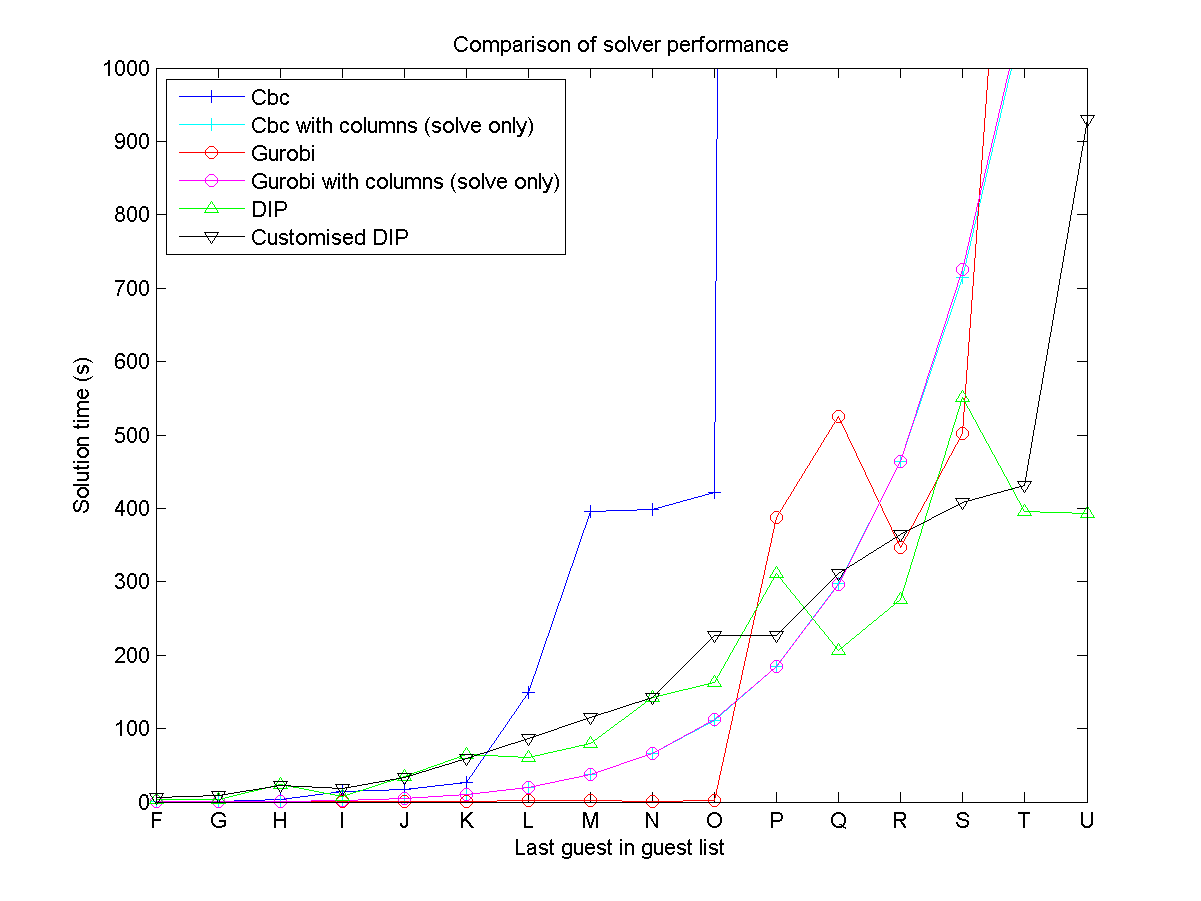
\includegraphics[bb=0 0 1201 901,scale=0.335]{compare.png}
\caption{Comparing solver performance on the Wedding Planner problem} \label{fig:compare}
\end{figure}
Thus, Dippy and \ac{DIP} not only provide a vastly simplified way to experiment with advanced \ac{MILP} techniques, they provide a better solver for problems in which column generation is the preferred approach.

Dippy presents the best of both worlds. It provides a mathematical modelling framework that makes it easy to quickly formulate \ac{MILP} problems. It also makes it easy to quickly customise the \ac{MILP} solution framework to experiment with the effectiveness of advanced \ac{MILP} techniques for the problem being solved. We have used Dippy successfully to enable final year undergraduate students to experiment with advanced branching, cut generation, column generation and root/node heuristics. Dippy also provides a simple interface to \ac{DIP}, a state of the art, ``out of the box'' column generation solver. Dippy breaks down the barrier to the experimentation with and use of advanced \ac{MILP} approaches for both practitioners and researchers. This enables them to concentrate on furthering Operations Research knowledge and solve hard problems instead of spending time programming \ac{MILP} formulations in a low-level language.

\newpage
\section{Acknowledgments}

The authors would like to thank Matt Galati, one of the authors of \ac{DIP}, for his help throughout this project and the Department of Engineering Science at the University of Auckland for their support of Qi-Shan and Iain during this research project.
\\
\\
\\
\vspace*{-0.5\baselineskip}
%\bibliographystyle{amsalpha}
%\bibliographystyle{plainnat}
\bibliographystyle{plain}
\bibliography{master}

\end{document}



